\documentclass[runningheads,a4paper]{llncs}

\usepackage[utf8]{inputenc}
\usepackage[OT1]{fontenc}
\usepackage[english]{babel}

\usepackage{amsmath}
\usepackage{amsfonts}
\usepackage{amssymb}
%\usepackage{amsthm}
\usepackage{amssymb}
\usepackage{bm}

%\usepackage{natbib}
%\usepackage[style=numeric]{biblatex}
%\addbibresource{boatpaper}
%\renewcommand{\bibfont}{\small}
%\renewcommand{\finentrypunct}{}

\usepackage[usenames,dvipsnames]{xcolor}
\usepackage{booktabs}
\usepackage{graphicx}
\usepackage{epsfig}
\usepackage{etoolbox}
\usepackage{url}
\usepackage[bookmarks]{hyperref}

\setcounter{tocdepth}{3}

\newcommand{\keywords}[1]{\par\addvspace\baselineskip
\noindent\keywordname\enspace\ignorespaces#1}


%%%%%%%%%%%%%%%%%%%%%%%%%%%%%%%%%%%%%%%%%%%%%%%%%%%%%%%%%%%%%%%%%%%%%%%%%%%%%%%%
%% Definitions
%%%%%%%%%%%%%%%%%%%%%%%%%%%%%%%%%%%%%%%%%%%%%%%%%%%%%%%%%%%%%%%%%%%%%%%%%%%%%%%%

\def\pdc{prior-data conflict}

\newcommand{\reals}{\mathbb{R}}
\newcommand{\posreals}{\reals_{>0}}
\newcommand{\posrealszero}{\reals_{\ge 0}}
\newcommand{\naturals}{\mathbb{N}}

\newcommand{\dd}{\,\mathrm{d}}

\newcommand{\mbf}[1]{\mathbf{#1}}
\newcommand{\bs}[1]{\boldsymbol{#1}}
\renewcommand{\vec}[1]{{\bm #1}}

\newcommand{\btheta}{\bs{\theta}}
\newcommand{\bpsi}{\bs{\psi}}
\newcommand{\bbeta}{\bs{\beta}}
\newcommand{\balpha}{\bs{\alpha}}

\newcommand{\uz}{^{(0)}} % upper zero
\newcommand{\un}{^{(n)}} % upper n
\newcommand{\ui}{^{(i)}} % upper i
\newcommand{\uinfty}{^{(\infty)}} % upper infty

\newcommand{\ul}[1]{\underline{#1}}
\newcommand{\ol}[1]{\overline{#1}}

\def\yz{y\uz}
\def\yn{y\un}
\def\yi{y\ui}

\def\yzl{\ul{y}\uz}
\def\yzu{\ol{y}\uz}

\def\ynl{\ul{y}\un}
\def\ynu{\ol{y}\un}

\def\yil{\ul{y}\ui}
\def\yiu{\ol{y}\ui}

\def\nz{n\uz}
\def\nn{n\un}
\def\ni{n\ui}

\def\nzl{\ul{n}\uz}
\def\nzu{\ol{n}\uz}

\def\nnl{\ul{n}\un}
\def\nnu{\ol{n}\un}

\def\nil{\ul{n}\ui}
\def\niu{\ol{n}\ui}

\def\taux{\tau(x)}
\def\ttau{\tilde{\tau}}
\def\ttaux{\ttau(x)}

\def\pz{\psi\uz}
\def\pn{\psi\un}

\def\Y{\mathcal{Y}}
\def\YZ{\Y\uz}
\def\YN{\Y\un}
\def\YI{\Y\ui}
\def\N{\mathcal{N}}
\def\NZ{\N\uz}
\def\NN{\N\un}
%\def\PZ{\text{I}\!\Pi\uz}
\def\PZ{I\!\!\Pi\uz}
%\def\PN{\text{I}\!\Pi\un}
\def\PN{I\!\!\Pi\un}
%\def\Pinfty{\text{I}\!\Pi\uinfty}
\def\MZ{\mathcal{M}\uz}
\def\MN{\mathcal{M}\un}

\newcommand{\az}{\alpha\uz}
\newcommand{\an}{\alpha\un}
\newcommand{\bz}{\beta\uz}
\newcommand{\bn}{\beta\un}

\def\Eta{\mathrm{H}}
\def\EZ{\mathrm{H}\uz}
\def\EN{\mathrm{H}\un}

\newcommand{\ez}{\eta_0}
\newcommand{\eo}{\eta_1}

\def\ezl{\ul{\eta}_0}
\def\ezu{\ol{\eta}_0}

\def\ezz{\eta_0\uz}
\def\ezn{\eta_0\un}
\def\eoz{\eta_1\uz}
\def\eon{\eta_1\un}

\def\ezzl{\ul{\eta}_0\uz}
\def\ezzu{\ol{\eta}_0\uz}
\def\eznl{\ul{\eta}_0\un}
\def\ezzn{\ol{\eta}_0\un}

\def\eozl{\ul{\eta}_1\uz}
\def\eozu{\ol{\eta}_1\uz}
\def\eonl{\ul{\eta}_1\un}
\def\eonu{\ol{\eta}_1\un}

\def\eol{\ul{\eta}_1}
\def\eou{\ol{\eta}_1}

\def\czl{\ul{c}\uz}
\def\czu{\ol{c}\uz}

\def\cnl{\ul{c}\un}
\def\cnu{\ol{c}\un}

\newcommand{\cdf}{\operatorname{F}}
\newcommand{\p}{\operatorname{P}}
\newcommand{\q}{\operatorname{Q}}
\newcommand{\E}{\operatorname{E}}
\newcommand{\V}{\operatorname{Var}}
\newcommand{\med}{\operatorname{med}} % Median
\newcommand{\modus}{\operatorname{mode}} % Mode
\newcommand{\logit}{\operatorname{logit}} % logit

%\DeclareMathOperator*{\argmin}{arg\,min}
%\DeclareMathOperator*{\argmax}{arg\,max}

\def\El{\ul{\E}}
\def\Eu{\ol{\E}}

\def\Pl{\ul{\p}}
\def\Pu{\ol{\p}}

\newcommand{\ber}{\operatorname{Ber}}   % Bernoulli Distribution
\newcommand{\bin}{\operatorname{Binom}} % Binomial Distribution
\newcommand{\be}{\operatorname{Beta}}   % Beta Distribution
\newcommand{\B}{\operatorname{B}}   % Beta Function



%%%%%%%%%%%%%%%%%%%%%%%%%%%%%%%%%%%%%%%%%%%%%%%%%%%%%%%%%%%%%%%%%%%%%%%%%%%%%%%%
%% Manuscript body
%%%%%%%%%%%%%%%%%%%%%%%%%%%%%%%%%%%%%%%%%%%%%%%%%%%%%%%%%%%%%%%%%%%%%%%%%%%%%%%%


\begin{document}

\mainmatter  % start of an individual contribution

% first the title is needed
\title{Sets of Prior Distributions\\ for Reflecting Prior-Data Conflict\\ and Strong Prior-Data Agreement}

% a short form should be given in case it is too long for the running head
\titlerunning{Sets of Priors for Reflecting Prior-Data Conflict and Agreement}

% the name(s) of the author(s) follow(s) next
%
% NB: Chinese authors should write their first names(s) in front of
% their surnames. This ensures that the names appear correctly in
% the running heads and the author index.
%
\author{Gero Walter\inst{1}%
\thanks{Gero Walter was supported by the Dinalog project
``Coordinated Advanced Maintenance and Logistics Planning for the Process Industries'' (CAMPI).}%
\and Frank P.A.\ Coolen\inst{2}}
%
%\authorrunning{Lecture Notes in Computer Science: Authors' Instructions}
% (feature abused for this document to repeat the title also on left hand pages)

% the affiliations are given next; don't give your e-mail address
% unless you accept that it will be published
\institute{%
School of Industrial Engineering,\\
Eindhoven University of Technology, Eindhoven, NL\\
\url{g.m.walter@tue.nl}
\and
Department of Mathematical Sciences,\\
Durham University, Durham, UK\\
\url{frank.coolen@durham.ac.uk}
}

%
% NB: a more complex sample for affiliations and the mapping to the
% corresponding authors can be found in the file "llncs.dem"
% (search for the string "\mainmatter" where a contribution starts).
% "llncs.dem" accompanies the document class "llncs.cls".
%

\maketitle


\begin{abstract}
Bayesian inference allows to combine observations with %(possibly subjective)
prior knowledge in the reasoning process.
The choice of a particular prior distribution to represent the available prior knowledge is, however,
often debatable, especially when prior knowledge is limited or data are scarce,
as then posterior inferences are highly dependent on the choice of prior.
Robust Bayesian analysis accounts for this issue by
inquiring whether posterior inferences change substantially
when the prior distribution is varied within a set of distributions that contains all `reasonable' priors.
Similar, but slightly different in scope, is the imprecise probability approach,
formalising the idea that sets of probability distributions
%(or, equivalently, interval-valued previsions or sets of desirable gambles)
should be taken to model prior knowledge more acurrately.
Imprecise probability allows to model prior-data conflict sensitivity:
%Models have been proposed where the ranges of posterior inferences
%are substantially larger when prior and data are in conflict.
Ranges of posterior inferences should be substantially larger when prior and data are in conflict.
Here we propose a new method for generating parameter prior sets in a conjugate setting
that, in addition to prior-data conflict sensitivity, allow to reflect \emph{strong prior-data agreement},
i.e., the case when prior and data coincide especially well, by increased posterior precision.
Although presented here for the case of binary data only,
it is easily extensible to the general exponential family case.
\keywords{Bayesian inference, strong prior-data agreement, prior-data conflict, imprecise probability, conjugate priors}
\end{abstract}


\section{Introduction}

The Bayesian approach to inference (see, e.g., \cite{2007:robert,2005:ruggeri}) %\cite[see, e.g.,][]{2007:robert,2005:ruggeri} 
offers the advantage to combine data and prior knowledge in a unified reasoning process.
The prior knowledge, i.e., information extraneous to data, is usually provided in the form of expert knowledge.
%
Bayesian inference usually starts with defining a parametric \emph{sample model},
denoted by $f(\vec{x} \mid \vartheta)$,
a conditional distribution of data $\vec{x} = (x_1, \ldots, x_n)$ given the value for a parameter $\vartheta$.
Prior information is then encoded by a so-called \emph{prior distribution} $p(\vartheta)$,
expressing the expert's opinion on probable values of $\vartheta$.
In light of the sample $\vec{x}$, the prior distribution is updated by Bayes' Rule
to obtain the so-called \emph{posterior distribution}
\begin{align}
\label{eq:bayesrule}
p(\vartheta\mid\vec{x}) &= \frac{f(\vec{x}\mid\vartheta) p(\vartheta)}{\int f(\vec{x}\mid\vartheta) p(\vartheta) \dd \vartheta}
                         \propto f(\vec{x}\mid\vartheta) \cdot p(\vartheta)\,.
\end{align}
The posterior distribution is understood to comprise all information from the sample and the prior knowledge.
It therefore underlies all further inferences on the parameter $\vartheta$,
like point estimators, interval estimators,
or predictions.
%or the \emph{posterior predictive distribution},
%giving the distribution of further observations based on the posterior.

However, the choice for the prior distribution to encode the given expert knowledge is often debatable,
and a specific choice of prior is difficult to justify.
A way to deal with this is to employ sensitivity analysis,
i.e., studying the effect of different choices of prior distribution on the quantities of interest.
This idea has been explored in systematic sensitivity analysis, or robust Bayesian methods;
for an overview on this approach, see, e.g.,
\cite{1994:berger} or \cite{2000:rios}. %\citeNP{2005:ruggeri}, \citeNP{2000:bergerinsuaruggeri}

The work we present here can be seen as belonging to the robust Bayesian approach, as our work uses sets of priors.
However, our focus and interpretation is slightly different,
as we consider the result of our procedure, sets of posterior distributions, as the proper result,
while a robust Bayesian would base his analyses on a single posterior from the set
in case (s)he was able to conclude that quantities of interest are not `too sensitive' to the choice of prior.
In contrast, our viewpoint is rooted in the theory of imprecise or interval probability \cite{itip,1991:walley},
where sets of distributions are used to express the precision of probability statements themselves:
the smaller the set of posteriors, the more precise the probability statements.

A central idea in imprecise probability is that the magnitude of a set of distributions,
and, in turn, the width of probability ranges based on it,
should reflect the precision of probabilistic knowledge.
A situation for which this relation should hold in particular is \emph{\pdc}:
% from abstract esrelpaper
%A problem that can arise in Bayesian inference is called prior-data conflict:
From the viewpoint of the prior $p(\vartheta)$, the observed data $\vec{x}$ seem very surprising,
i.e., information from data is in conflict with prior assumptions (see, e.g., \cite{2006:evans}). %\cite[see, e.g.,][]{2006:evans}.
This is most relevant when there is not enough data to overrule the prior;
as it is then unclear whether to put more trust to prior assumptions or to the observations,
posterior inferences should clearly reflect this state of uncertainty.
\cite{Walter2009a} pointed out that
both precise and imprecise models based on conjugate priors can be insensitive to prior-data conflict.

For Bayesian inference based on a single, precise conjugate prior,
learning from data amounts to averaging between prior and data
(see, e.g., \cite[\S~1.2.3.1]{2013:diss-gw}).
%as will be illustrated in Sect.~\ref{sec:beta-binom}.
While this averaging property allows for great tractability,
it is also at the root of prior-data conflict insensitivity: 
When observed data are very much different from what is assumed in the prior,
this conflict is simply averaged out,
and is not reflected in the variance of the posterior,
ultimately conveying a false sense of certainty:
A posterior with small variance indicates that we know what's going on quite precisely -- but in case of \pdc\ we in fact do not.

Prior-data conflict is instead reflected by a larger set of posteriors,
i.e., more cautious probability statements,
when using carefully tailored sets of conjugate priors,
as suggested by \cite{Walter2009a}.
In this approach, sets of conjugate priors are defined via sets of canonical parameters,
and conditions for the shape of these parameter sets were derived that ensure \pdc\ sensitivity.
\cite{Walter2009a} then suggested a parameter set shape
that balances tractability and ease of elicitation
with desired inference properties.
The approach has since been successfully applied in common-cause failure modelling \cite{Troffaes2014a}
and system reliability \cite{2015:walter}.

In the present paper, we want to further refine this approach
by complementing the increased imprecision reaction to \pdc\
with a `bonus' in precision for the case when prior and data coincide especially well,
a situation that we will call \emph{strong prior-data agreement}.
In terms of the discussion at the end of \cite[\S~3.1.4]{2013:diss-gw},
we thus sacrifice a bit of tractability through employing a more complex parameter set shape
in order to obtain improved model behaviour.%
%\footnote{Some first results in this direction were already presented in \cite[\S~A.2]{2013:diss-gw}.}

The present work presents an idea how to define, through a novel parameter set shape,
sets of priors such that the correpsonding sets of posteriors
show both \pdc\ sensitivity and a reaction to strong prior-data agreement.
%***motivation: clever choice of prior sets
%***emphazise that this is basically an idea for defining sets of priors***
To keep things simple, we restrict ourselves here to the case of the Beta-Binomial model (see Sect.~\ref{sec:beta-binom}),
but the approach is generalizable to arbitrary canonical conjugate priors,
and we will comment on this in the concluding remarks (Sect.~\ref{sec:concluding}).

\cite{Walter2009a} used a parametrization 
that allows for an intuitive interpretation of the parameters of the Beta distribution
and clearly shows that the update step from prior to posterior
amounts to a weighted average in the conjugate setting (Sect.~\ref{sec:beta-binom}).
The new shape is instead defined in terms of another parametrization
which was recently suggested by Bickis \cite{2015:mik-isipta}.
We will therefore briefly characterise this novel parametrisation of canoncial conjugate priors (Sect.~\ref{sec:miksworld}),
%this approach relies on.
and then go on to suggest a shape in this parametrisation that accomplishes
both \pdc\ sensitivity and `bonus precision' in case of strong prior-data agreement.
We propose a parametric description for such a shape
and show that it indeed leads to the desired properties (Sect.~\ref{sec:boatshape}).
Section~\ref{sec:concluding} concludes the paper by discussing generalizations and potential applications. 


\section{The Beta-Binomial Model in Two Parametrizations}
\label{sec:beta-binom}

Consider an experiment where there are only two possible outcomes,
\emph{success} and \emph{failure}, and success arising with some probability $p$.
The number of successes $s$ in a series of $n$ independent trials
has then a Binomial distribution with parameters $p$ and $n$,
where $n$ is known but $p \in [0,1]$ is unknown.
In short, $S\mid p \sim \bin(n,p)$, which means
\begin{align}
f(s\mid p) &= P(S = s \mid p) = {n \choose s} p^s (1-p)^{n-s},\quad s \in \{0, 1, \ldots, n\}\,.
\label{eq:binompmf}
\end{align}
In a Bayesian setting, information about unknown parameters (here, $p$) is then expressed
by a so-called prior distribution, here $f(p)$, usually derived from expert information.
In general, the posterior distribution according to Bayes' rule is hard to obtain,
especially due to the integral in the denominator of \eqref{eq:bayesrule}.
The posterior can be approximated with numerical methods,
for example the Laplace approximation, or simulation methods like MCMC (Markov chain Monte Carlo).

However, Bayesian inference not necessarily entails complex calculations and simulation methods.
With a clever choice of parametric family for the prior distribution,
the posterior distribution belongs to the same parametric family as the prior, just with updated parameters.
Such prior distributions are called \emph{conjugate} priors.
Basically, with conjugate priors one trades flexibility for tractability:
The parametric family restricts the form of the prior pdf,
but with the advantage of much easier computations.

The conjugate prior for the Binomial distribution \eqref{eq:binompmf} is the Beta distribution,
which is usually parametrized with parameters $\alpha > 0$ and $\beta > 0$,
\begin{align}
f(p\mid\alpha,\beta) &= \frac{1}{B(\alpha,\beta)}\, p^{\alpha-1}\, (1-p)^{\beta-1}\,,
\label{eq:betadensab}
\end{align}
where $B(\cdot,\cdot)$ is the Beta function.
In short, we write $p \sim \be(\alpha,\beta)$.
%$\alpha$ and $\beta$ can be interpreted as pseudocounts,
%giving the number of virtual successes and failures, respectively.
The combination of a Binomial sampling model with this conjugate Beta prior is called \emph{Beta-Binomial model},
and parameters identifying the prior distribution are often called \emph{hyperparameters}.

In the remainder of the paper, we will denote prior parameter values by an upper index~${}\uz$,
in contrast to posterior parameter values obtained after observing $n$ trials,
which are indicated by an upper index~${}\un$.
With this notational convention,
let $S\mid p \sim \bin(n,p)$ and $p \sim \be(\az,\bz)$.
Then it holds that $p \mid s \sim \be(\an,\bn)$,
where $\an$ and $\bn$ are updated, posterior parameters, obtained as
%\begin{align}
$\an = \az + s$ and $\bn= \bz + n - s$.
%\label{eq:betapostab}
%\end{align}
Note that $\az$ and $\bz$ can be interpreted as pseudocounts,
forming a hypothetical sample with $\az$ sucesses and $\bz$ failures.

We will consider now a different parametrisation of the Beta distribution
which is more useful when we generalize to sets of priors. % we find more intuitive
It is defined as
%\begin{align}
$\nz = \az + \bz$, $\yz = \frac{\az}{\az+\bz}$.
%\label{eq:betareparam}
%\end{align}
Writing $p \sim \be(\nz,\yz)$ thus corresponds to
%\begin{align}
%$f(p\mid\nz,\yz) = \frac{p^{\nz\yz-1}\, (1-p)^{\nz(1-\yz)-1}}{B(\nz\yz,\nz(1-\yz))}$.
$f(p) \propto p^{\nz\yz-1}\, (1-p)^{\nz(1-\yz)-1}$.
%\label{eq:betadensny}
%\end{align}
$\nz > 0$ and $\yz \in (0,1)$ are sometimes called \emph{canonical} parameters,
identified from rewriting the density in canonical form;
see for example \cite[pp.~202 and 272f]{2000:bernardosmith}, or \cite[\S 1.2.3.1]{2013:diss-gw}.
(This canonical form gives a common structure to all conjugacy results in exponential families.)
%In this parametrisation, the updated, posterior parameters are given by
%\begin{align}
%\nn &= \nz + n\,, &
%\yn &= \frac{\nz}{\nz + n} \cdot \yz + \frac{n}{\nz + n} \cdot \frac{s}{n}\,.
%\label{eq:betapostny}
%\end{align}
%and we write $p\mid s \sim \be(\nn,\yn)$.
From the properties of the Beta distribution,
it follows that $\yz = \E[p]$ is the prior expectation for the functioning probability $p$,
and that larger $\nz$ values lead to greater concentration of probability mass around $\yz$,
since $\V(p) = \frac{\yz (1-\yz)}{\nz + 1}$.
Consequently, $\nz$ represents the prior strength
and moreover can be directly interpreted as a (total) pseudocount due to the relation $\nz = \az + \bz$.

The posterior given that $s$ out of $n$ components function,
written in terms of $\nz$ and $\yz$,
is a Beta distribution with updated parameters
\begin{align}
\nn &= \nz + n\,, &
\yn &= \frac{\nz}{\nz + n} \cdot \yz + \frac{n}{\nz + n} \cdot \frac{s}{n}\,.
\label{eq:nyupdate}
\end{align}
Thus, after observing $s$ successes in $n$ trials,
the posterior mean $\yn$ for $p$ is a weighted average of
the prior mean $\yz$ and $s/n$ (the observed fraction of successes),
with weights $\nz$ and $n$, respectively.
So $\nz$ takes on the same role for the prior mean $\yz$
as the sample size $n$ does for the observed mean $s/n$,
confirming its interpretation as a pseudocount.

The parametrization in terms of prior mean and prior strength (or pseudocount)
makes clear that in this conjugate setting,
learning from data corresponds to averaging between prior and data.
This form is attractive because it enhances the interpretability of the model and prior specification,
and makes Bayesian inference easily tractable.
However, it also makes clear what should be a serious concern in any Bayesian analysis:
when observed data differ greatly from what is expressed in the prior,
this conflict is simply averaged out
and is not reflected in the posterior or posterior predictive distributions.


\section{Generalized Bayesian Inference with Sets of Beta Priors}
\label{sec:setsofbetapriors}

As was shown by \cite{Walter2009a}, %Walter \& Augustin (2009),
it is possible obtain a meaningful reaction to prior-data conflict while retaining tractability
by using sets of priors $\MZ$ produced through parameter sets $\PZ = [\nzl, \nzu] \times [\yzl, \yzu]$.
%(a detailed discussion of different choices for $\PktZ$ is given in \citet[\S 3.1]{2013:diss-gw}.)
More generally, \cite[\S 3.1]{2013:diss-gw} describes a framework for
Bayesian inference using sets of conjugate priors based on arbitrary parameter sets $\PZ$.
%This sets of priors approach also allows to model vague and incomplete expert knowledge.
Applying this framework to the Beta-Binomial model described above,
each prior parameter pair $(\nz, \yz) \in \PZ$ corresponds to a Beta prior,
so one may take $\MZ$ directly as a set of Beta priors.
Alternatively, one may take the convex hull of all Beta priors with $(\nz, \yz) \in \PZ$ as $\MZ$,
i.e., $\MZ$ consists of all finite mixtures of Beta priors with $(\nz, \yz) \in \PZ$.

It is a modeling decision whether to take $\MZ$ as containing only Beta priors or also the mixtures.
In the first case, bounds for any inferences can be obtained by optimizing over $\PZ$.
In the second case, optimizing over $\PZ$ will only yield bounds for all inferences
that are \emph{linear functions} of $\nz$ and $\yz$,
as the linearity ensures that bounds must correspond to the extreme points of the convex set of priors,
which are the Beta priors with $(\nz, \yz) \in \PZ$.
For inferences not linear in $\nz$ and $\yz$, meaningful bounds might not exist.%
\footnote{Consider for example the prior variance for $p$, $\V(p) = \frac{\yz (1-\yz)}{\nz + 1}$,
being nonlinear in $\nz$ and $\yz$.
It is intuitively clear that $\V(p)$ can be larger for mixture distributions than for `pure' Beta distributions.}

In both cases, the set of posteriors $\MN$ is obtained by updating each prior in $\MZ$ according to Bayes' Rule.
This element-by-element updating can be rigorously justified
as ensuring coherence \cite[\S 2.5]{1991:walley}, and was termed ``Generalized Bayes' Rule'' by Walley \cite[\S 6.4]{1991:walley}.
In the first case, $\MN$ is a set of Beta distributions with parameters $(\nn, \yn)$,
obtained by updating $(\nz, \yz) \in \PZ$ according to \eqref{eq:nyupdate},
leading to the set of updated parameters
\begin{align}
\PN &= \Big\{ (\nn, \yn) \mid (\nz, \yz) \in \PZ = [\nzl, \nzu] \times [\yzl, \yzu] \Big\}\,.
\label{eq:paramsets}
\end{align}
In the second case, the set of Beta distributions corresponding to $(\nn, \yn) \in \PN$
forms the extreme points of the convex set of posteriors $\MN$,
such that, just like $\MZ$, $\MN$ can be described as a set of all finite mixtures of Beta distributions,
but now with $(\nn, \yn) \in \PN$, see \cite[pp.~56f]{2013:diss-gw}.

The set of posteriors $\MN$ forms the basis for all inferences,
leading to probability \emph{ranges} obtained by optimizing over $\MN$.
As a running example, in the Beta-Binomial model %as discussed in Section~\ref{sec:beta-binom},
the posterior predictive probability %$[\lpr,\upr]$
for the event that a future single draw is a success is equal to $\yn$, and so we get,
for an imprecise model $\MZ$ based on $\PZ$,
the lower and upper probability
\begin{align*}
\inf_{\PN} \yn &= \inf_{\PZ} \frac{\nz\yz + s}{\nz +n} & &\text{and} &
\sup_{\PN} \yn &= \sup_{\PZ} \frac{\nz\yz + s}{\nz +n}\,.
\end{align*}

The relation between $\PZ$ and $\MZ$, as well as between $\PN$ and $\MN$,
allows to characterize model properties through properties of $\PZ$ and $\PN$,
as is done in \cite[\S 3.1.2 -- 3.1.4]{2013:diss-gw}.
In particular, specific imprecise probability models are obtained by certain choices of $\PZ$.
The well-known Imprecise Dirichlet Model \cite{1996:walley::idm}
corresponds to a choice of $\PZ = \nz \times (\yzl, \yzu)$ where $(\yzl, \yzu) = (0,1)$.
The model proposed by \cite{2005:quaeghebeurcooman} generally assumes $\PZ = \nz \times [\yzl, \yzu]$,
and was shown to be insensitive to prior-data conflict by \cite{Walter2009a},
who proposed parameter sets $\PZ = [\nzl, \nzu] \times [\yzl, \yzu]$ instead.

%*** lower, upper $\yn$ \& range for QdC, rectangle, discuss some inference properties.
Indeed, with $\PZ = \nz \times [\yzl, \yzu]$, we have $\PN = \nn \times [\ynl, \ynu]$, where
\begin{align*}
\ynl &= \frac{\nz\yzl + s}{\nz + n} & &\text{and} &
\ynu &= \frac{\nz\yzu + s}{\nz + n}\,.
\end{align*}
The posterior imprecision in the $y$ dimension, denoted by $\Delta_y(\PN)$, is 
\begin{align*}
%\label{eq:deltay}
\Delta_y(\PN) &= \ynu - \ynl = \frac{\nz (\yzu - \yzl)}{\nz +n}\,,
\end{align*}
and so the same for any fixed $n$, independent of $s$.
In contrast, parameter sets $\PZ = [\nzl, \nzu] \times [\yzl, \yzu]$
provide prior-data conflict sensitivity, since
%\footnote{See \cite{Walter2009a} or \cite[\S 3.1.4]{2013:diss-gw} for more details.}
\begin{align*}
%\label{eq:deltay2}
\Delta_y(\PN) &= \frac{\nzu (\yzu - \yzl)}{\nzu + n} %\nonumber\\
               + \inf_{\yz \in [\yzl,\yzu]} |s/n - \yz| \frac{n (\nzu - \nzl)}{(\nzl + n)(\nzu + n)}\,.
\end{align*}

As discussed at the end of \cite[\S 3.1.4]{2013:diss-gw},
the shape of $\PZ$ thus poses a trade-off:
Less complex shapes are easy to handle and lead to tractable models,
but will offer less flexibility in expressing prior information
and may have undesired inference properties.
In contrast, more complex shades may allow for more sophisticated model behaviour
at the cost of more complex handling.


\section{A Third Parametrization for Beta Priors}
\label{sec:miksworld}

In the parametrization in terms of $\nz$ and $\yz$ as described in Sect.~\ref{sec:beta-binom},
a conjugate Beta prior is updated to its respective posterior by a shift in the parameter space,
given by rewriting \eqref{eq:nyupdate}:
\begin{align*}
\nz &\mapsto \nz + n\,, &
\yz &\mapsto %\frac{\nz}{\nz + n} \cdot \yz + \frac{n}{\nz + n} \cdot \frac{s}{n} = 
             \yz + \frac{s - n \yz}{\nz+n}\,.
\end{align*}
We see thus that, while the shift for the $n$ coordinate is the same for all elements $(\nz,\yz)$ of $\PZ$,
the shift in the $y$ coordinate depends on $\nz$, $n$, $s$, and the location of $\yz$ itself
(namely, how far $\yz$ is from $s/n$).
Due to this, the shape of $\PZ$ changes during the update step.
This shape change from $\PZ$ to $\PN$ is problematic for understanding of the update step in generalized Bayesian inference,
as its effects on posterior inferences are difficult to grasp.

Therefore, to isolate the influence of a set shape,
we now consider a different parametrisation of the prior
where each coordinate has the same shift in updating.
The updating of a parameter set
then corresponds to a shift of the entire set within the parameter space.
This parametrization has recently been developed by Bickis \cite{2015:mik-isipta}. %Mi\c{k}elis Bickis
In this novel parametrization, a prior is represented by a coordinate $(\ezz,\eoz)$,
where $\eoz$ replaces $\yz$, while $\ezz$ is just a shifted version of $\nz$.
%there, update step for $\nz$ is the same, and shift for parameter replacing $\yz$ is the same for all. 
To keep things simple, we will not describe its derivation here (this is described in detail in \cite{2015:mik-isipta}),
and present it in relation to $(\nz, \yz)$:
%\begin{equation}
\begin{align}
\label{eq:trafotony}
%\begin{aligned}
\nz &= \ezz + 2\,, &
\yz &= \frac{\eoz}{\ezz + 2} + \frac{1}{2}\,.
%\end{aligned}
%\end{equation}
\end{align}
The domain of $\eta_0$ and $\eta_1$ in case of the Beta-Binomial model is
\begin{align}
\label{eq:eta-domain}
\Eta &= \Big\{ (\eta_0,\eta_1) \Big| \eta_0 > -2,\ |\eta_1| < \frac{1}{2}(\eta_0 + 2) \Big.\Big\}\,,
\end{align}
and the update step in terms of $\eta_0$ and $\eta_1$ is given by
\begin{equation}
\label{eq:eta-update}
\begin{aligned}
\eta_0\un &= \eta_0\uz + n\,, & 
\eta_1\un &= \eta_1\uz + \frac{1}{2}(s - (n-s)) = \eta_1\uz + s - \frac{n}{2}\,.
\end{aligned}
\end{equation}
%where $s$ is again the number of successes in the $n$ Bernoulli trials.
Each success thus
leads to a step of $1$ in the $\eta_0$ direction and of $+\frac{1}{2}$ in the $\eta_1$ direction,
while each failure
leads to a step of $1$ in the $\eta_0$ direction and of $-\frac{1}{2}$ in the $\eta_1$ direction. %
%\footnote{We will treat $s$ as a a real-valued observation in $[0,n]$
%because the continuous representation is convenient for our discussions,
%keeping in mind that in reality it can only take integer values.}
%\begin{figure}  %trim=l b r t
%\centering
%\fbox{%
%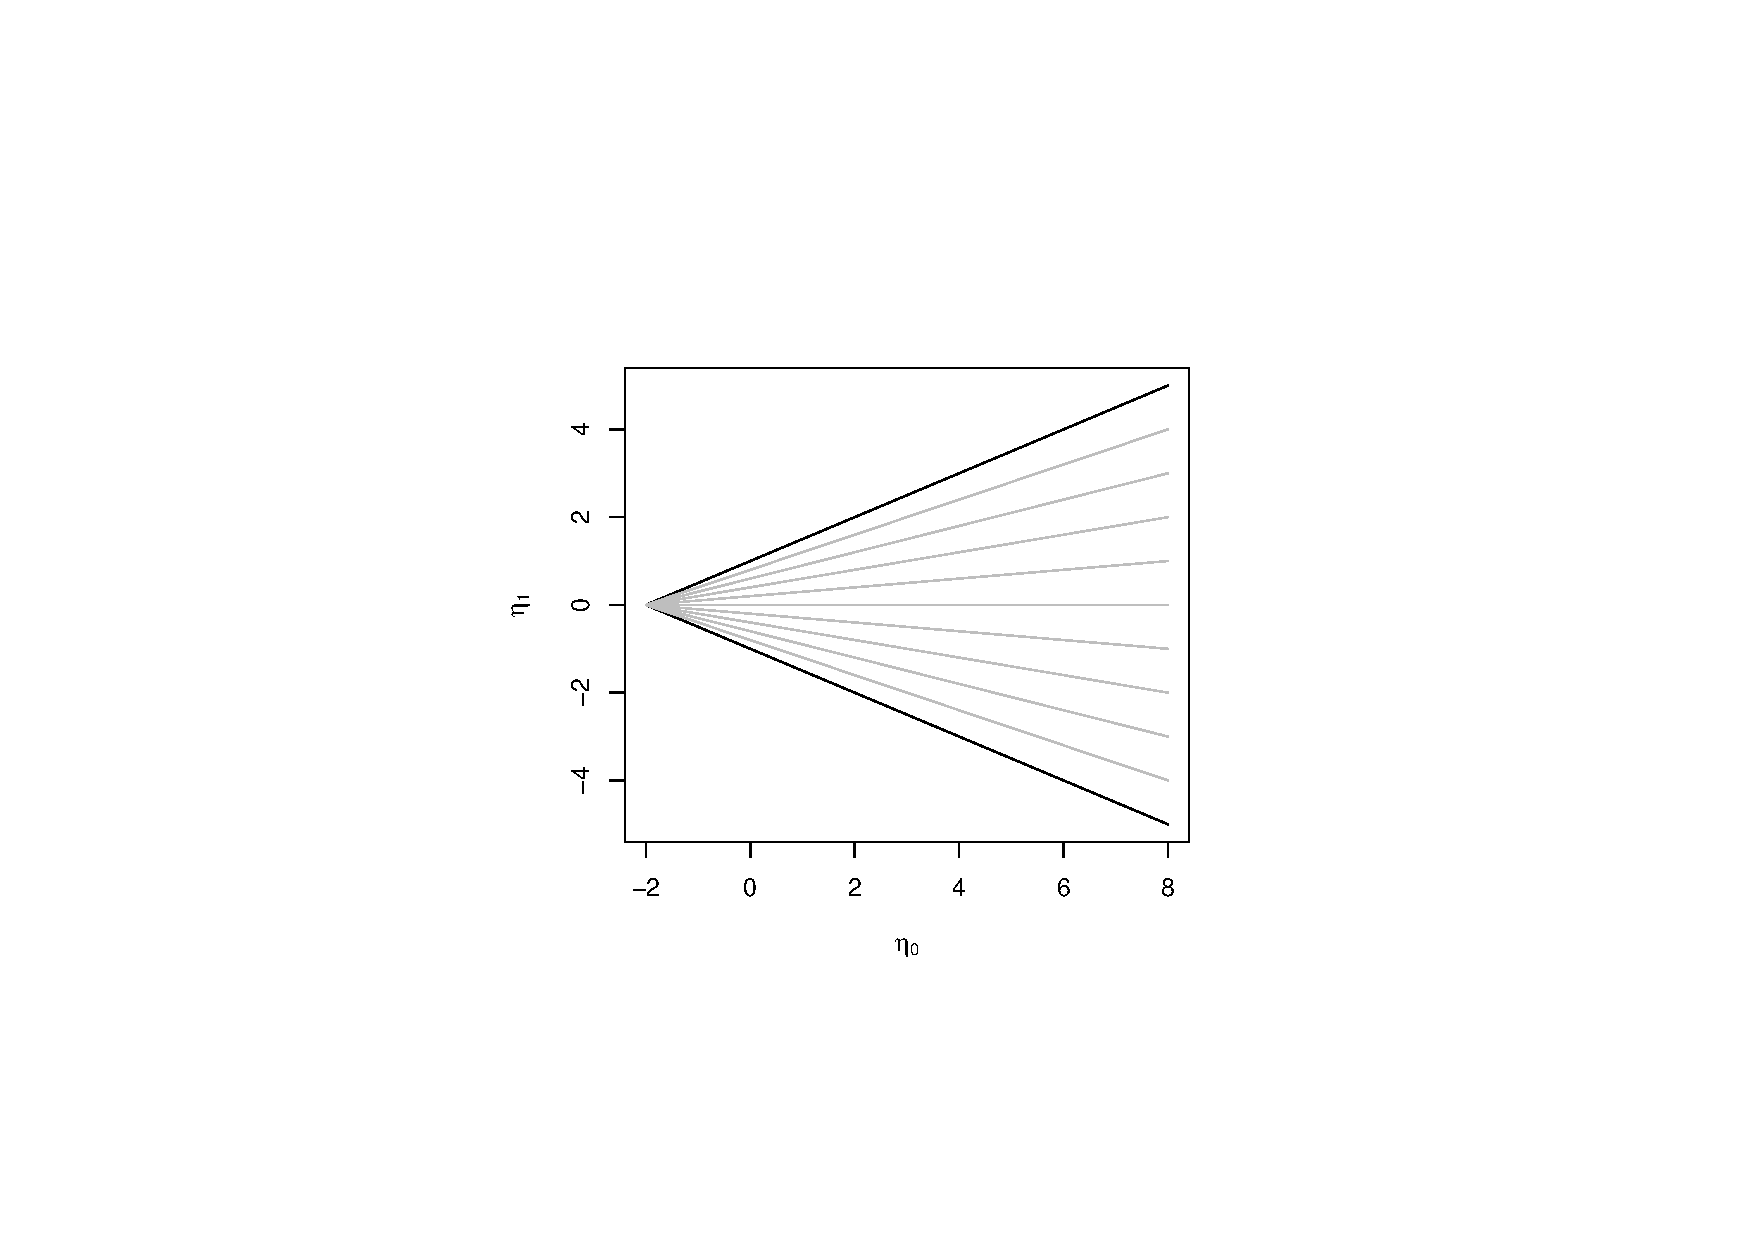
\includegraphics[trim = 86mm 48mm 94mm 62mm, clip, width=0.5\textwidth]{R/boatshape-domain}%
%}
%\caption[Bounds for the domain of $\eta_0$ and $\eta_1$ for the Beta-Binomial model,
%with rays of constant expectation for $y_c = \{0.1,0.2,\ldots,0.9\}$.]%
%{Bounds for the domain of $\eta_0$ and $\eta_1$ for the Beta-Binomial model (black),
%with rays of constant expectation for $y_c = \{0.1,0.2,\ldots,0.9\}$ (grey).}
%\label{fig:boatshape-domain}
%\end{figure}

While $\yz$ had the convenient property of being equal to
the prior expectation of the mean sample statistic $s/n$,
$\eta_1$ is only slightly more difficult to interpret.
From \eqref{eq:trafotony} we can derive that points $(\eta_0,\eta_1) \in \Eta$
on rays emanating from the coordinate $(-2,0)$,
i.e., coordinates satifying
\begin{align}
\label{eq:raysofconstantexpectation}
\eta_1 &= (\eta_0 + 2)(y_c - 1/2) 
\end{align}
will have a constant expectation of $y_c$.
The domain $\Eta$, and these \emph{rays of constant expectation} emanating from the coordinate $(-2,0)$,
can be seen in Fig.~\ref{fig:boatshape-vertical}.

In the parametrisation in terms of $(\nz,\yz)$,
posterior inferences based on $\yn$ become more precise with increasing $n$
because $\Delta_y(\PN) \to 0$ for $n \to \infty$.
In the domain $\Eta$, %as depicted in Figure~\ref{fig:boatshape-domain},
instead the rays of constant expectation fan out for growing $n$,
while a parameter set will retain its size in updating.
Increased precision in a posterior parameter set $\EN$, which is just
its prior counterpart $\EZ$ shifted to the right,
is given by the fact that the more $\EN$ is located to the right,
the fewer rays of constant expectation $\EN$ it will intercept.
Imprecision in terms of $\yn$
can thus be imagined as the size of the `shadow' that a set $\EN$ casts
when considering a light source in $(-2,0)$. %(the point from which the rays of constant expectation emanate).
The smaller this shadow, the more precise the inferences.
In terms of the $(\nz, \yz)$ parametrization, we will denote the bounds of this shadow by $\ynl$ and $\ynu$:
\begin{align*}
\ynl &:= \min_{(\ezn,\eon) \in \EN} \frac{\eon}{\ezn+2} + \frac{1}{2}\,, &
\ynu &:= \max_{(\ezn,\eon) \in \EN} \frac{\eon}{\ezn+2} + \frac{1}{2}\,.
\end{align*}
We call the $\ez$ coordinate of $\arg\min_{(\eta_0,\eta_1) \in \EN} \yn$ and $\arg\max_{(\eta_0,\eta_1) \in \EN} \yn$
the \emph{lower} and \emph{upper touchpoint} of $\EN$ responsible for the shadow $[\ynl, \ynu]$.
Mutatis mutandis, the same definitions can be made for the prior set $\EZ$.

Due to the fanning out of rays, most shapes for $\EZ$ will lead to decreasing imprecision for increasing $n$.
Indeed, models with $\PZ = \nz \times [\yzl, \yzu]$
are represented here again by a line segment $\EZ = \ezz \times [\eozl,\eozu]$.
%such that the lower and upper posterior touchpoint is at $\ezn$, for any $s$ and $n$.
Defining $\eonl$ and $\eonu$ as the updated versions of $\eozl$ and $\eozu$, respectively,
we get $\eonu-\eonl = \eozu-\eozl$,
so imprecision decreases here because a line segment of fixed size
will cast a smaller shadow when further to the right,
as illustrated in Fig.~\ref{fig:boatshape-vertical}.
\begin{figure}  %trim=l b r t
\centering
%\fbox{%
%\includegraphics[trim = 16mm 48mm 25mm 62mm, clip, width=\textwidth]{R/boatshape-vertical2}%
\includegraphics[trim = 2mm 6mm 10mm 20mm, clip, width=0.8\textwidth]{R/boatshape-vertical2}%
%}
\caption[Line segment parameter set $\EZ$ %
and respective posterior sets for $s/n=0.5$ and $s/n=0.9$.]%
%{Bounds for the domain of $\eta_0$ and $\eta_1$ for the Beta-Binomial model (black),
%with rays of constant expectation for $y_c = \{0.1,0.2,\ldots,0.9\}$ (grey).}
{Prior parameter set $\EZ = \ezz \times [\text{\underline{$\eta$}${}_1\uz$},\eozu]$
and respective posterior sets $\EN$ for $s/n=0.5$ (left) and $s/n=0.9$ (right).
Bounds for the domain $\Eta$ are in black, with rays of constant expectation for $y_c = \{0.1,0.2,\ldots,0.9\}$ in grey. 
Note that all sets have the same size, imprecision decreasing only through their position on the $\eta_0$ axis.}
\label{fig:boatshape-vertical}
\end{figure}

For \pdc\ sensitivity, we need shapes that cover a range of $\eta_0$ values,
just like we needed sets with a range of $\nz$ values to ensure this property.
Sets that are elongated along a certain ray of constant expectation
will behave here similar to the rectangular shapes of Sect.~\ref{sec:setsofbetapriors}.
When shifted along its ray of constant expectation,
imprecision will be reduced as the shadow of the set will become smaller just as described above for line segments.
When such a shape is instead shifted away from its ray of constant expectation,
imprecision will increase, as a prolonged shape that is now turned away from its ray 
will cast a larger shadow (see Fig.~\ref{fig:boatshape-posterior-mik} below).%
%\footnote{This will become clear from the depiction of boatshape sets in Figure~\ref{fig:boatshape-posterior-mik}.} 
%A set $\EZ$ allowing for more precison in case of strong prior-data agreement
%must thus be able to cast a smaller shadow if the update shift is along the direction of its ray.
%of $s/n$ according the information,


\section{The Boatshape}
\label{sec:boatshape}

The shape for $\EZ$ that we suggest to obtain both \pdc\ sensitivity and increased precision
in case of strong prior-data agreement looks like a bullett, or like a boat with a transom stern
(see, e.g., Fig.~\ref{fig:boatshape-posterior-mik} below), hence its name.
The curvature along its length in the direction of its constant rays of expectation
leads to smaller $\Delta_y(\PN)$ as compared to a rectangular $\PZ$ with the same prior range $\Delta_y(\PZ)$,
as illustrated in Fig.~\ref{fig:boatshape-posterior-normal}.

The strong prior-data agreement effect is realized
through the touchpoints determining $\ynl$ and $\ynu$
moving along the shape during updating,
%being attained at higher values of $\eta_0$ for larger $n$,
as will be demonstrated in Sect.~\ref{sec:spda-property}.
This is advantageous when considering that the spread of the Beta posteriors is determined by $\eta_0 = \nz - 2$.
In case of strong prior-data agreement, variances in the `critical' distributions
at the boundary of the posterior expectation interval $[\ynl,\ynu]$ will thus be lower.
In particular, credible intervals for these `critical' distributions will be shorter, 
such that the union of all credible intervals for Beta distributions with $(\ezn, \eon) \in \EN$,
taken as a posterior inference reflecting uncertainty due to both vague prior knowledge and stochasticity, will be shorter.
%
%In the remainder of this section, 
%we will suggest a parametrisation for a curved shape in the $(\eta_0, \eta_1)$ space.
%The definition, along with some graphical examples, is given in Sect.~\ref{sec:basicdefboat},
%and we discuss a number of technical results for this shape in subsequent sections.


\subsection{Basic Definition}
\label{sec:basicdefboat}

We will now present a parametrisation for such a boat-shaped parameter set $\EZ$.
To keep things simple, we will consider here only prior sets
that are symmetric around the $\eta_0$ axis, i.e., centered around $y_c = 0.5$,
expressing the prior information that we deem a fraction of successes of $\frac{s}{n} = \frac{1}{2}$ as the most probable.
Sets $\EZ$ with central ray $y_c \neq 0.5$ can be obtained
by rotating the set around $(\eta_0, \eta_1) = (-2,0)$ such that $y_c$ forms the axis of symmetry.
All results for sets with $y_c = 0.5$ generalize straight-forwardly to the case $y_c \neq 0.5$;
a numerical example is given in Fig.~\ref{fig:ppp2}.

For the contours of $\EZ$, we suggest an exponential function as the functional form,
where the `prow' of the set is located at $(\ezl, 0)$.
The lower and the upper contour $\czl(\eta_0)$ and $\czu(\eta_0)$ are defined as
%\begin{align*}
%\czl(\eta_0) &= -a \left( 1 - e^{-b(\eta_0 - \ezl)} \right)\,, \\
%\czu(\eta_0) &= \phantom{-}%
%                 a \left( 1 - e^{-b(\eta_0 - \ezl)} \right)\,, 
%\end{align*}
\begin{align}
\czl(\eta_0) &= -a \left( 1 - e^{-b(\eta_0 - \ezl)} \right)\,, &
\czu(\eta_0) &=  a \left( 1 - e^{-b(\eta_0 - \ezl)} \right)\,, 
\label{eq:basiccontours}
\end{align}
where $a > 0$ and $b > 0$ are parameters controlling the shape of $\EZ$.
%We will also need the respective derivations with respect to $\eta_0$, given by
%\begin{align*}
%\frac{d}{d\eta_0} \czl(\eta_0) &= -ab e^{-b(\eta_0 - \ezl)}\,, \\
%\frac{d}{d\eta_0} \czu(\eta_0) &= \phantom{-}%
%                                   ab e^{-b(\eta_0 - \ezl)}\,.
%\end{align*}
Given parameters $\ezl$, $\ezu$, $a$, and $b$, $\EZ$ is thus defined as
\begin{align}
\label{eq:basicset}
\EZ =
\{(\eta_0,\eta_1) \colon \ezl \le \eta_0 \le \ezu, \czl(\eta_0) \le  \eta_1 \le \czu(\eta_0) \}\,.
\end{align}
A prior boatshape set with $\ezl=1$, $\ezu=6$, $a=1.5$, and $b=0.9$,
together with corresponding posterior sets for different observations,
is depicted in Fig.~\ref{fig:boatshape-posterior-mik}.
The same prior and posterior sets in terms of $(\nz, \yz)$ are depicted in Fig.~\ref{fig:boatshape-posterior-normal}.
%shown in terms of $(\eta_0,\eta_1)$ (left) and in terms of $(\nz, \yz)$ (right).
%\begin{figure}  %trim=l b r t
%\centering
%\fbox{%
%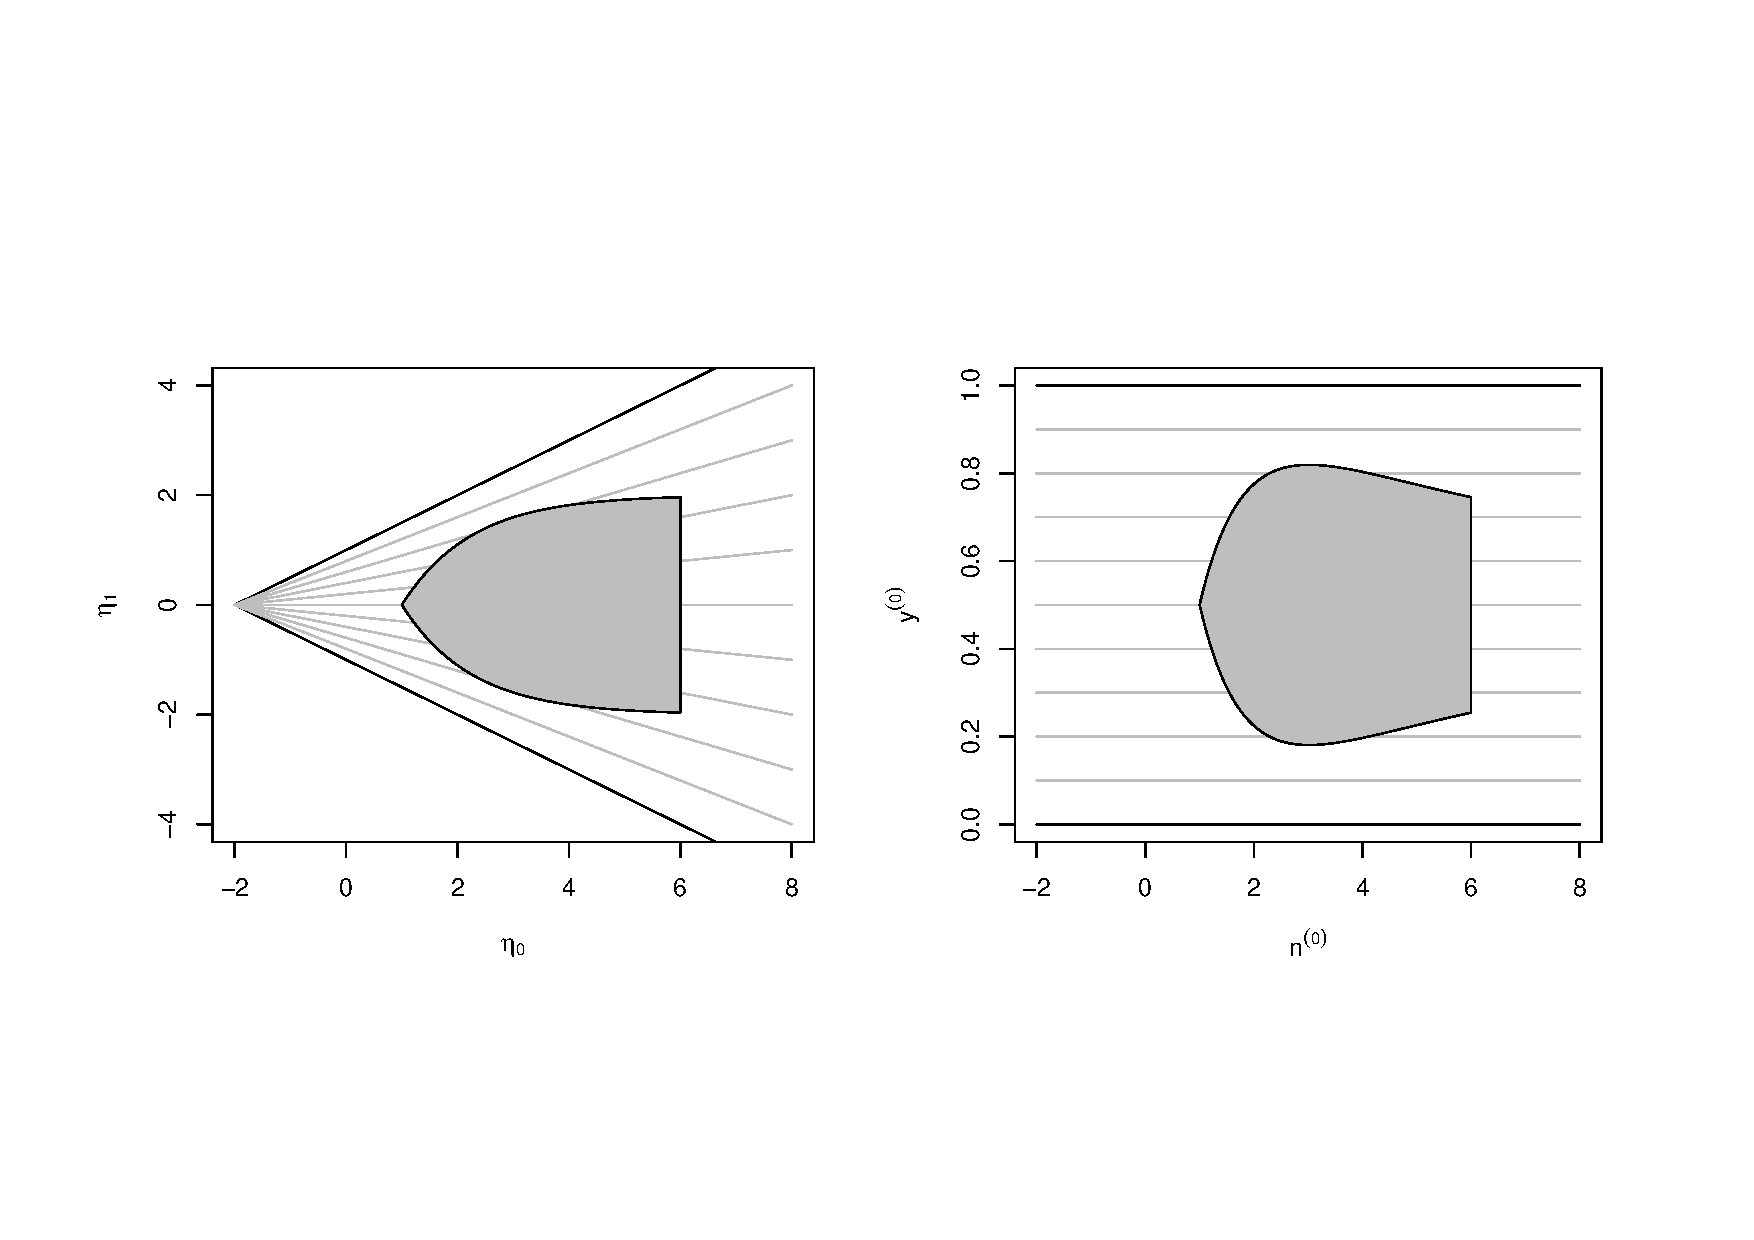
\includegraphics[trim = 15mm 45mm 25mm 60mm, clip, width=\textwidth]{R/boatshape-prior}%
%}
%\caption[Boatshape prior set in the parametrisation via $(\eta_0,\eta_1)$ and via $(\nz,\yz)$.]%
%{Boatshape prior set in the parametrisation via $(\eta_0,\eta_1)$ (left) and via $(\nz,\yz)$ (right),
%with parameters $\ezl=1$, $\ezu=6$, $a=2$, and $b=0.8$.}
%\label{fig:boatshape-prior}
%\end{figure}
\begin{figure}  %trim=l b r t
\centering
%\fbox{%
%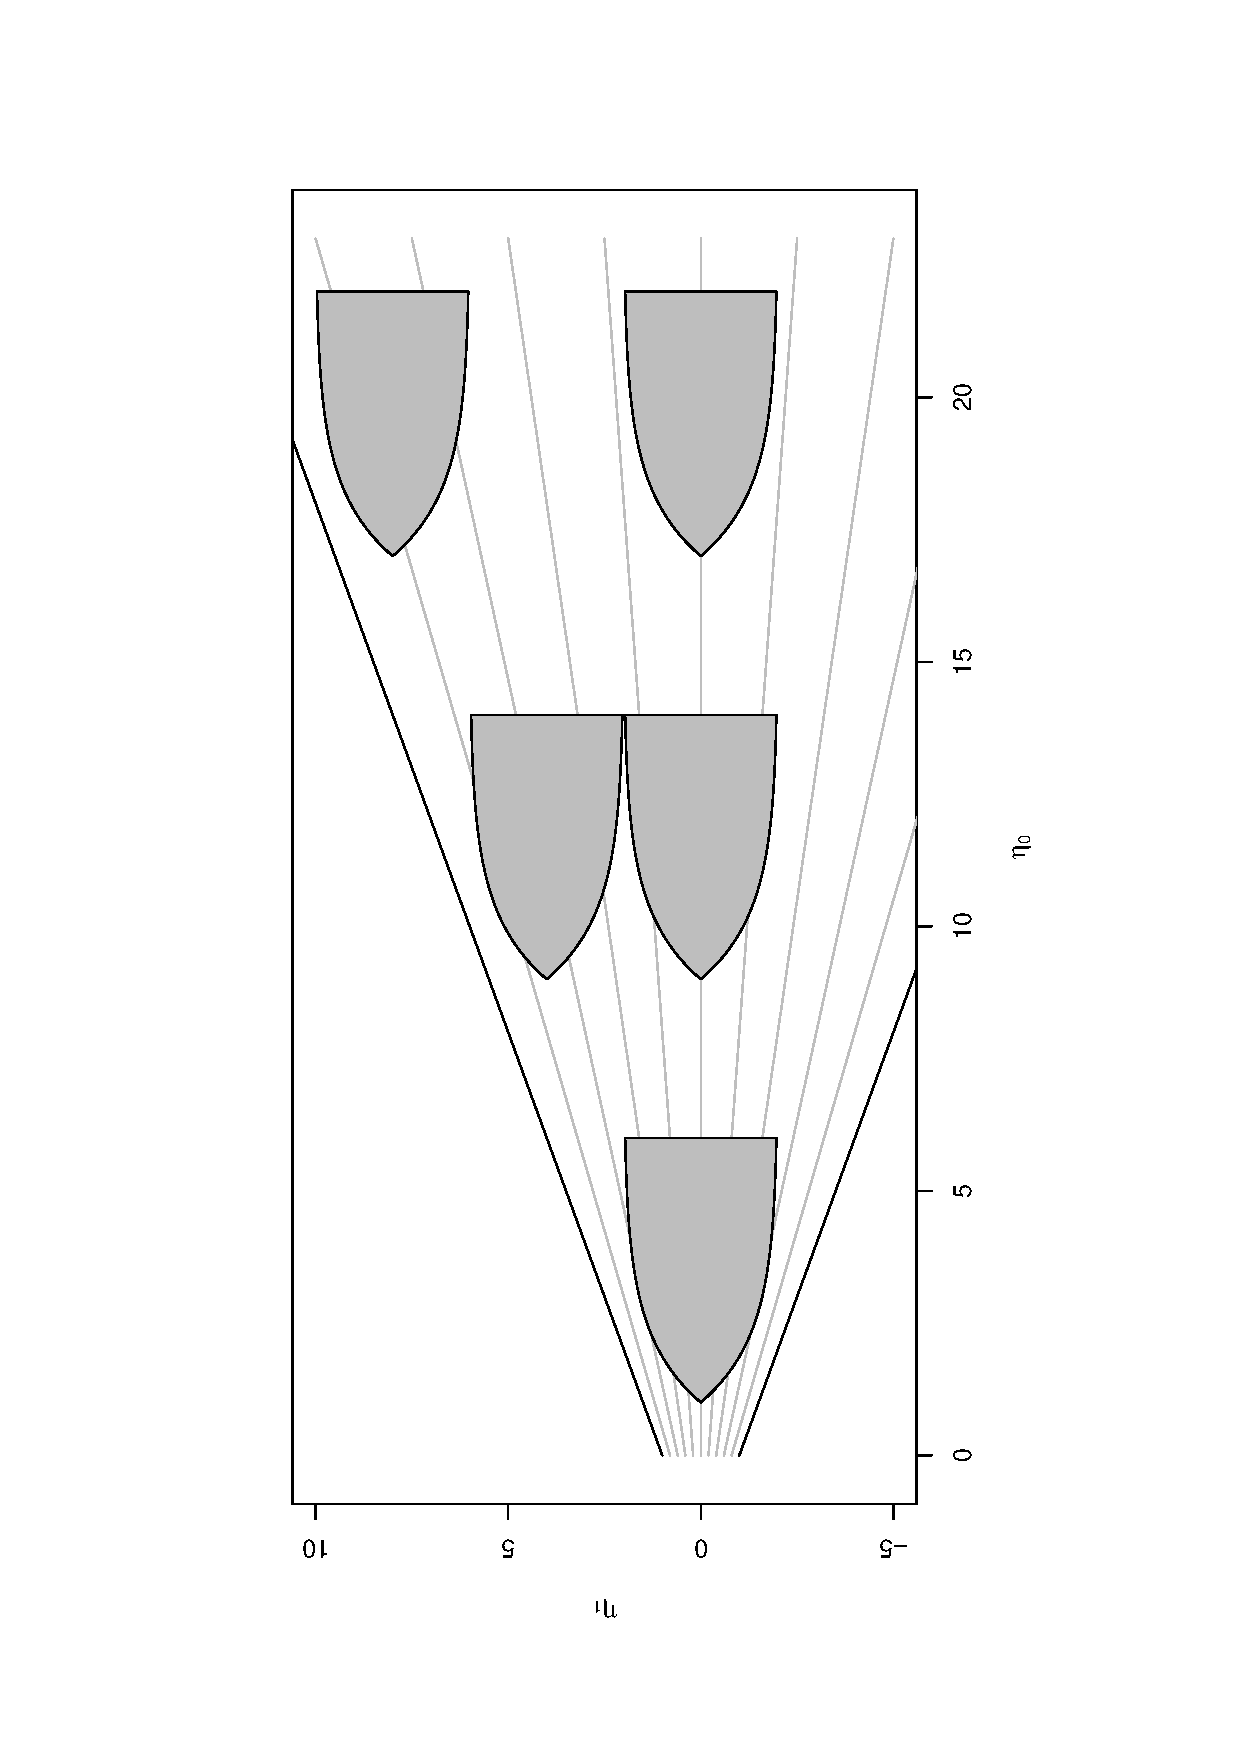
\includegraphics[trim = 20mm 35mm 30mm 45mm, clip, width=\textwidth]{R/boatshape-posterior-mik}%
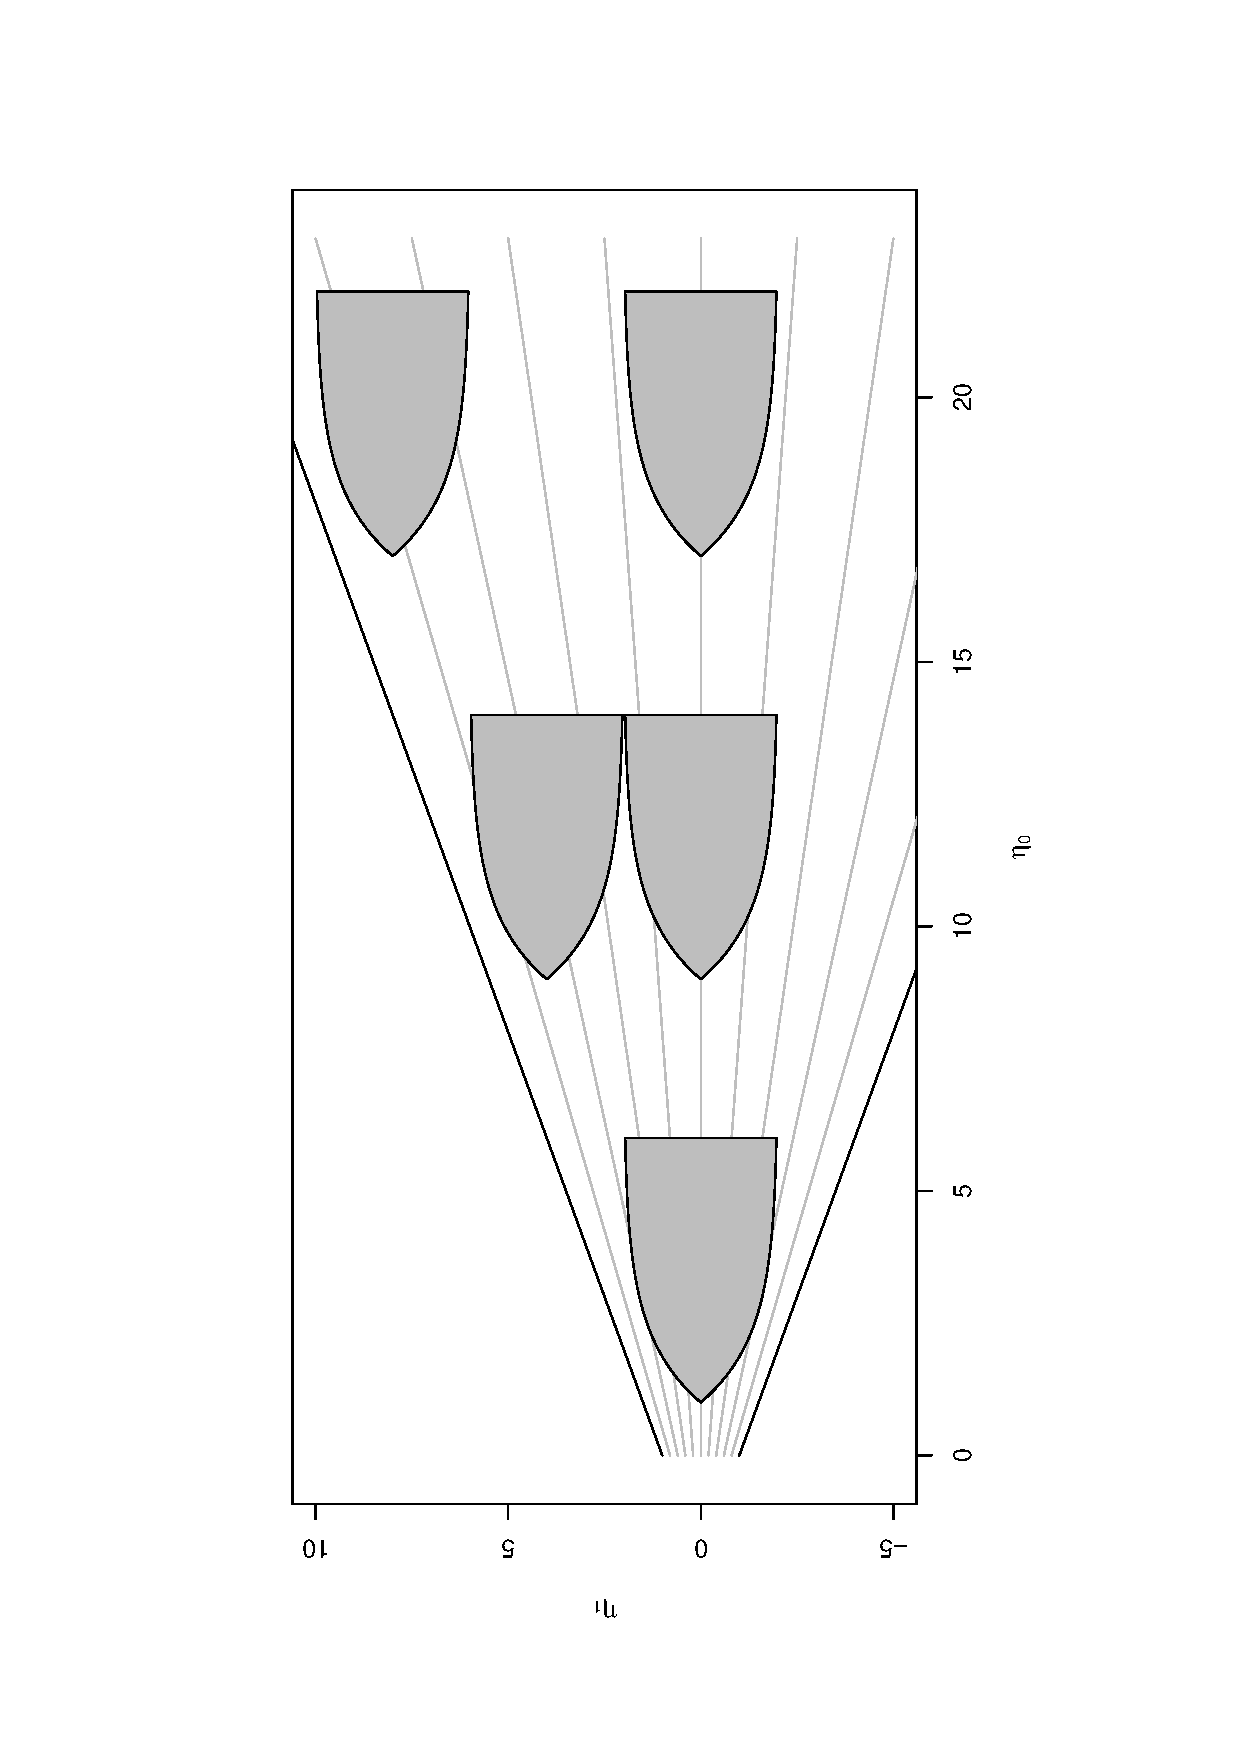
\includegraphics[width=\textwidth]{R/boatshape-posterior-mik}%
%}
\caption[Boatshape prior and posterior sets for data in accordance and in conflict with the prior set.]%
{Boatshape prior and posterior sets for data in accordance and in conflict with the prior set.
The parameters for the prior set are $\ezl=1$, $\ezu=6$, $a=1.5$, and $b=0.9$.
While the posterior sets for $\frac{s}{n}=0.5$ move along the ray for $y_c=0.5$,
the posterior sets for $\frac{s}{n}=1$ are shifted away from the ray for $y_c=0.5$,
resulting in increased posterior imprecision.
Note that lower and upper touchpoints are in the middle of the contour
for the prior set and the posterior sets resulting for data $\frac{s}{n}=0.5$,
while the lower touchpoint is at the end for the posterior sets for data $\frac{s}{n}=1$.}
%(See also Figure~\ref{fig:boatshape-posterior-normal}).}
\label{fig:boatshape-posterior-mik}
\end{figure}

We have as yet no appealing formal description for the role of the parameters $a$ and $b$. %that,
%togeher with $\ezl$ and $\ezu$, define the boat-set (see Section~\ref{sec:basicdefboat} below).
Informally, $a$ determines the half-width of the set;
the width, i.e., the size in the $\eta_1$ dimension, would be $a$ if $\ezu \to \infty$.
$b$ instead determines the `bulkyness' of the shape.
Together with $\ezl$, $a$ and $b$ determine the prior interval for the expected success probability $[\yzl, \yzu]$.
Increasing each of $\ezl$, $a$ and $b$ while keeping the other two fixed leads to a wider $[\yzl, \yzu]$.
%For fixed $\ezl$ and $a$, increasing $b$ leads to a wider prior expectation interval.
%For $[\yzl, \yzu]$, the choice of $\ezu$ is irrelevant.%
$\ezu$ plays only a role in determining when the `unhappy learning' phase starts
(see end of Sect.~\ref{sec:generalupdate}).
\begin{figure}  %trim=l b r t
\centering
%\fbox{%
%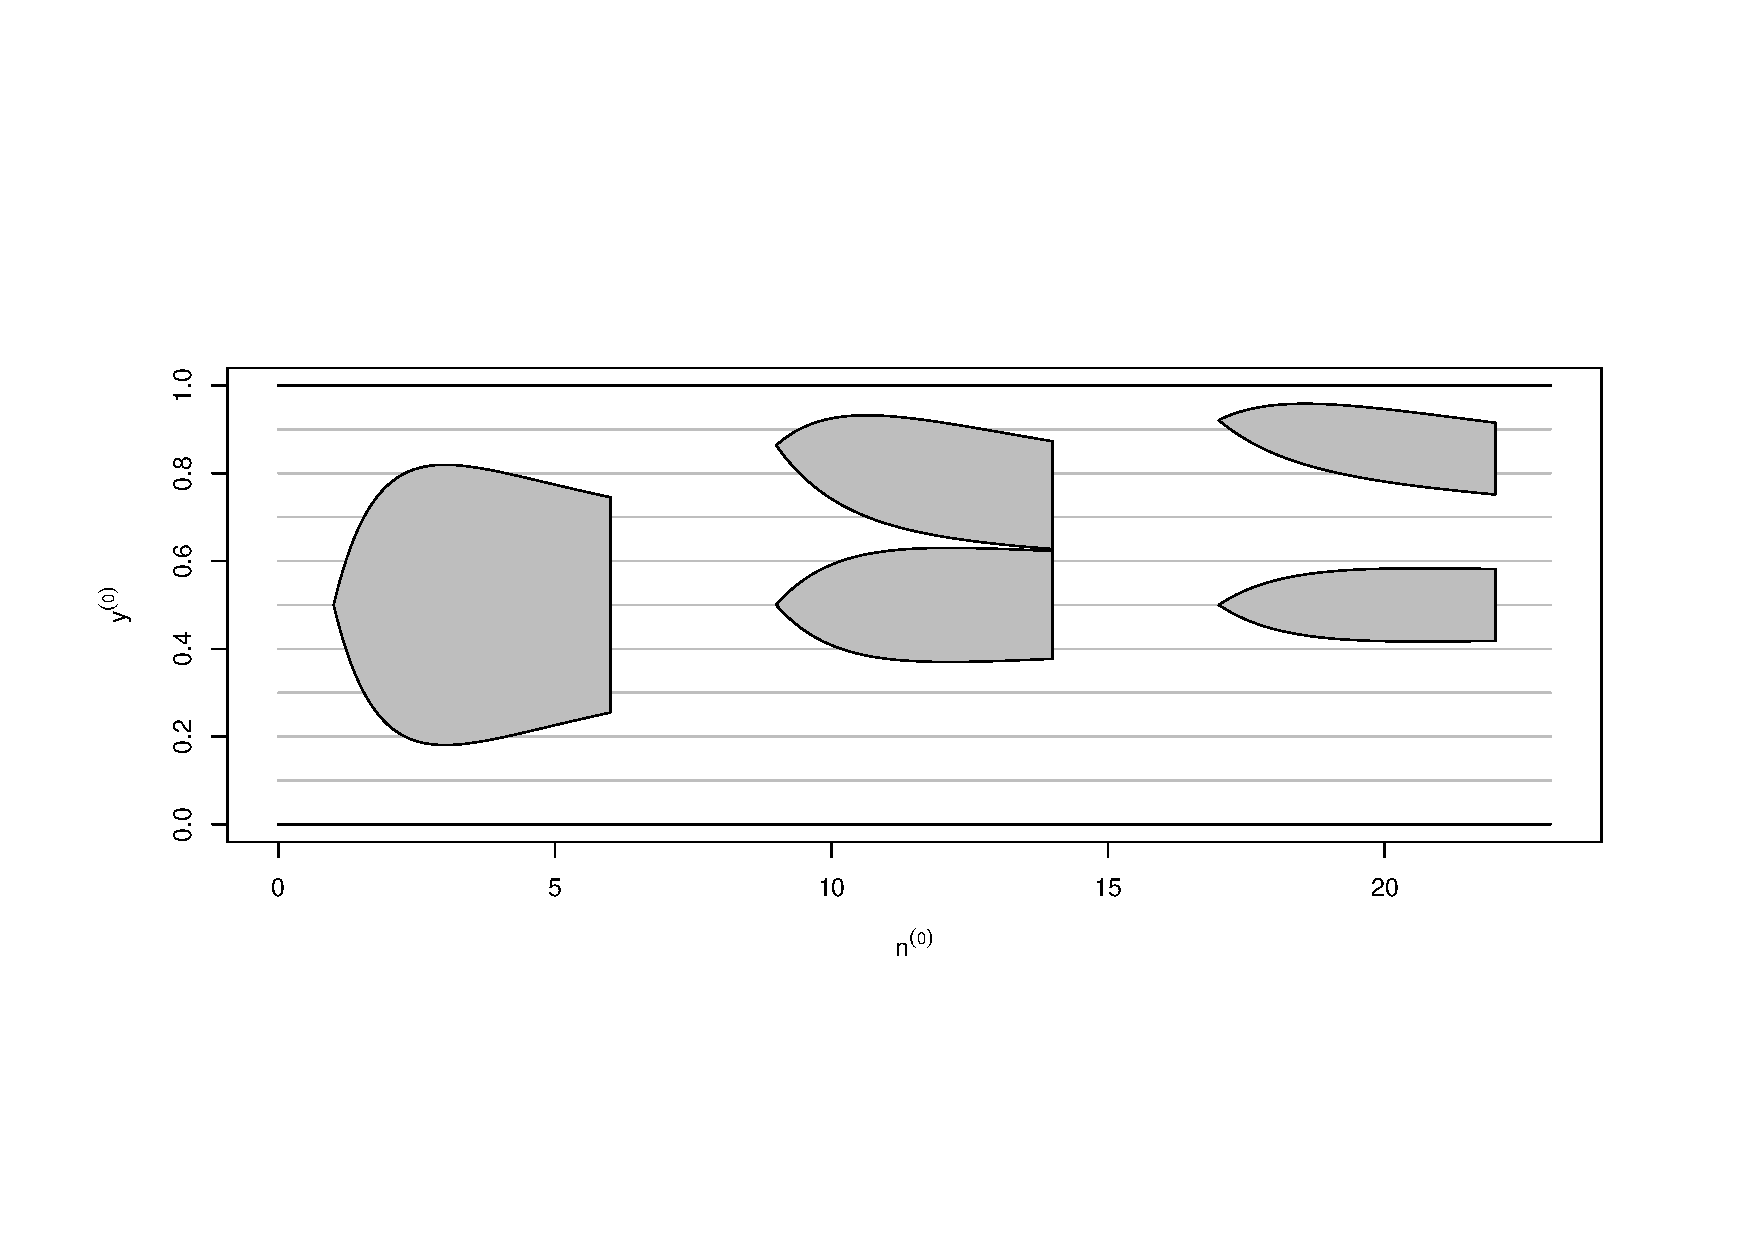
\includegraphics[trim = 15mm 45mm 25mm 60mm, clip, width=\textwidth]{R/boatshape-posterior-normal}%
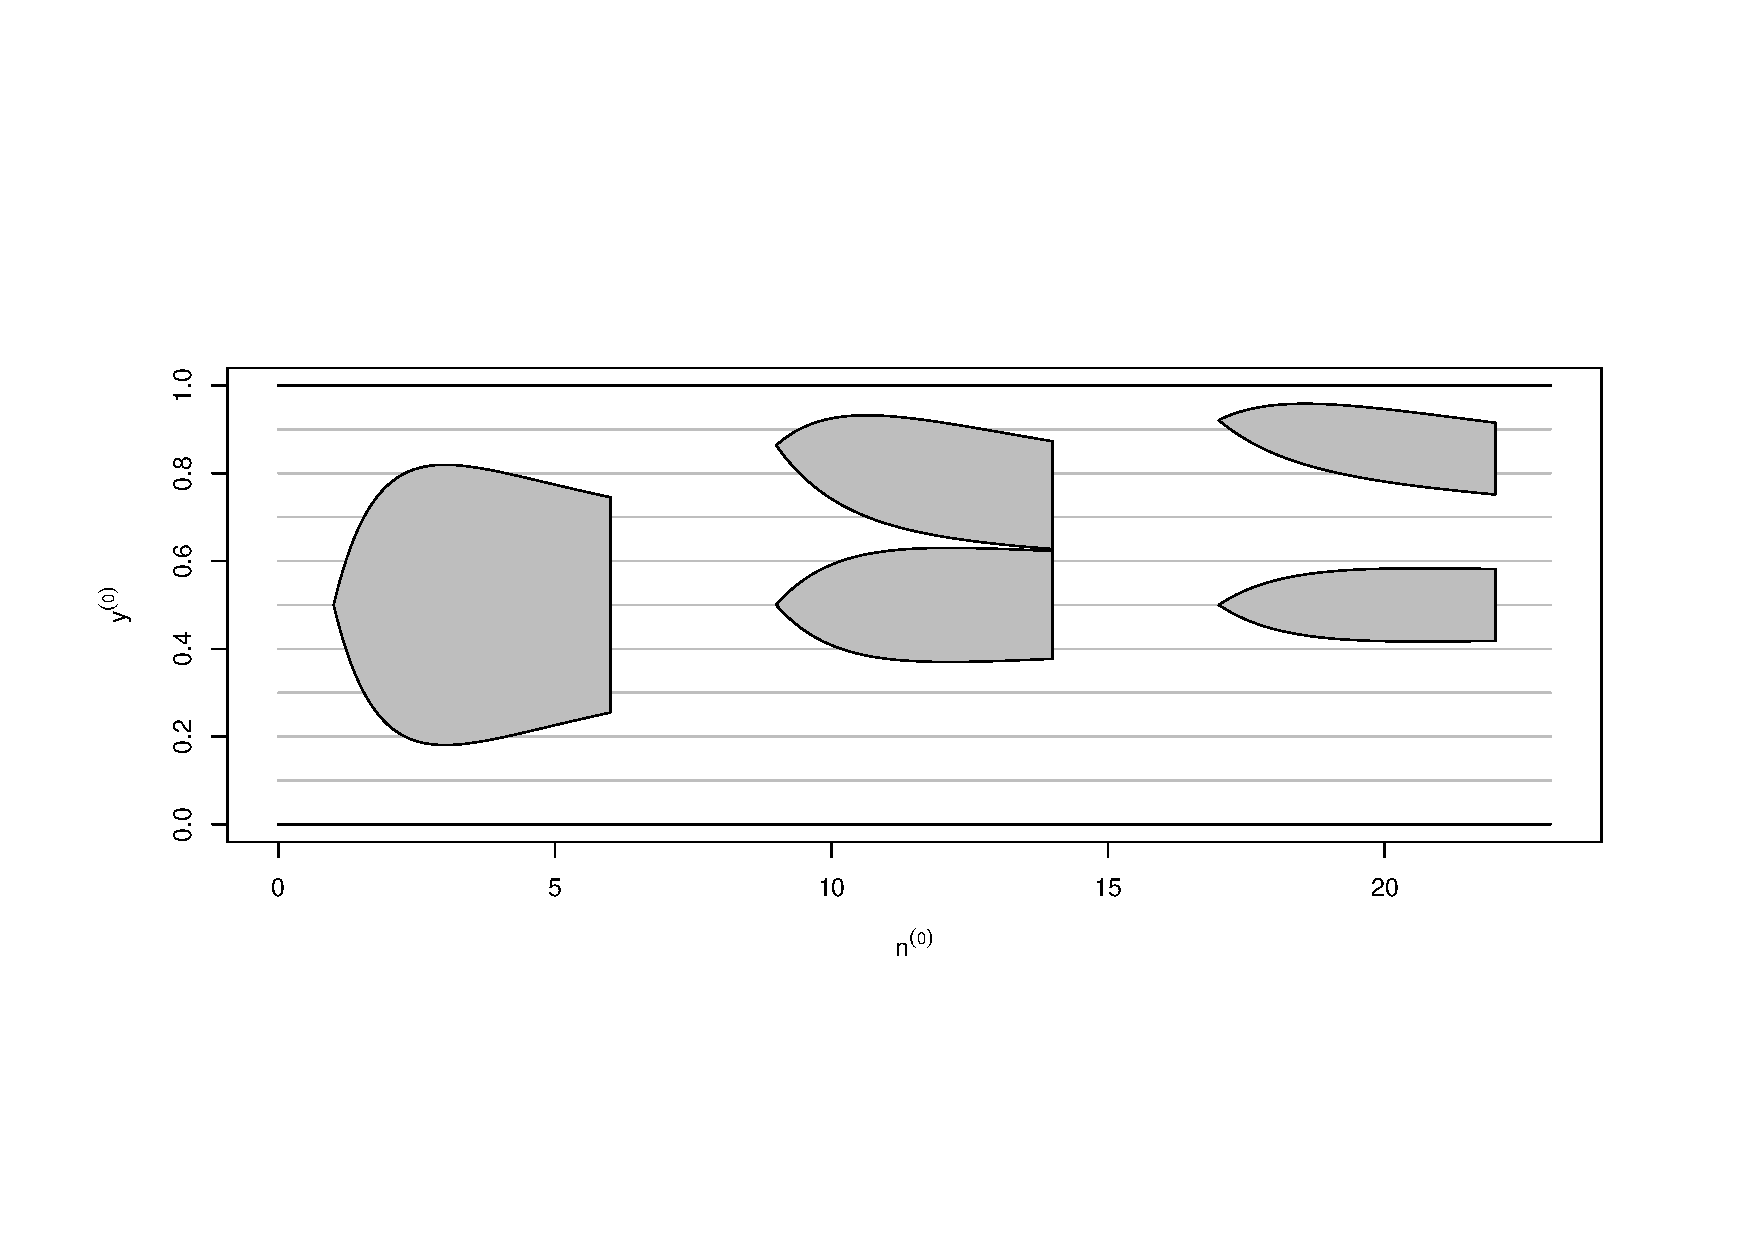
\includegraphics[width=\textwidth]{R/boatshape-posterior-normal}%
%}
\caption[Boatshape prior and posterior sets from Fig.~\ref{fig:boatshape-posterior-mik} in the $(\nz,\yz)$ parametrisation.]%
{Boatshape prior and posterior sets from Fig.~\ref{fig:boatshape-posterior-mik} in the $(\nz,\yz)$ parametrisation.
The rectangular prior set with the same range for $\yz$ as the prior boatshape set
and the corresponding posterior sets are drawn with dashed lines. 
Note that all posterior boatshape sets have shorter $\yn$ ranges than their corresponding posterior rectangle sets.}
\label{fig:boatshape-posterior-normal}
\end{figure}

We see from the prior set in Fig.~\ref{fig:boatshape-posterior-normal}
that the lower and the upper bound for $\yz$
is attained in the middle of the set contour.
To determine $\yzl$ and $\yzu$, we need to find the corresponding
touchpoints $\eta_0^{l(0)}$ and $\eta_0^{u(0)}$
by identifying the rays of constant expectation \eqref{eq:raysofconstantexpectation}
that are tangents to $\EZ$ and then solving for $\eta_0$.
Since $\EZ$ is symmetric to the $\eta_0$ axis, we have $\eta_0^{u(0)} = \eta_0^{l(0)}$,
and we will determine ${\eta_0^u}\uz$ by considering the upper contour tangent.
We get
\begin{align}
%a - a \big(1 + b(\eta_0^u + 2)\big) e^{-b(\eta_0^u - \ezl)} &\stackrel{!}{=} 0
%& &\Longleftrightarrow &
1 + b({\eta_0^u}\uz + 2) &\stackrel{!}{=} e^{b({\eta_0^u}\uz - \ezl)}\,.
\label{eq:eta0uprior}
\end{align}
This equation has only one solution for ${\eta_0^u}\uz > \ezl$
that is, however, not available in closed form.
Generally, the nearer ${\eta_0^u}\uz$ is to $\ezl$, the larger $\frac{d}{d\eta_0} \czu({\eta_0^u}\uz)$,
such that $\yzu$ %the upper expected value for the prior set
is further away from $\frac{1}{2}$.
This means that, for fixed $\ezl$ and $b$, the smaller ${\eta_0^u}\uz$, the more imprecise the prior parameter set.


\subsection{Strong Prior-Data Agreement Property}
\label{sec:spda-property}

We now derive the property that sets \eqref{eq:basicset}
lead to especially precise inferences when data are strongly supporting prior information
as the touchpoint moves further to the right in that case. %when updating with strong-agreement data.
The basic shape is symmetric around the $\ez$ axis ($\EZ$ has central ray $y_c = 0.5$),
and update with strong-agreement data $s/n = 0.5$ means that $\EZ$ is shifted along the $\ez$ axis by $n$,
such that also $\EN$ is symmetric around the $\ez$ axis.
We thus need to consider only one touchpoint.
With the upper prior touchpoint at ${\eta_0^u}\uz$,
the touchpoint movement to the right means that the upper posterior touchpoint ${\eta_0^u}\un$
is larger than the updated prior touchpoint,
so we need to show that ${\eta_0^u}\un > {\eta_0^u}\uz + n$.

The upper contour for the posterior boatshape,
updated with $s = \frac{n}{2}$, %has its `prow' now at $(\ezl + n, 0)$,
is $\czu$ from \eqref{eq:basiccontours} shifted to the right by $n$, i.e.,
%\begin{align*}
$\cnu(\eta_0) = a - a e^{-b(\eta_0 - n -\ezl)}$.
%\frac{d}{d\eta_0} \ol{c}(\eta_0) &= ab e^{-b(\eta_0 - n - \ezl)} \,.
%\end{align*}
The equation to identify the posterior upper touchpoint is then
\begin{align}
%a - a \big(1 + b({\eta_0^u}\un + 2)\big) e^{-b({\eta_0^u}\un - n - \ezl)} &\stackrel{!}{=} 0 \nonumber\\
1 + b({\eta_0^u}\un + 2) &\stackrel{!}{=} e^{b({\eta_0^u}\un - n - \ezl)} \,.
\label{eq:eta0uposterior}
\end{align}
Comparing \eqref{eq:eta0uposterior} to \eqref{eq:eta0uprior}, we can conclude
that indeed ${\eta_0^u}\un > {\eta_0^u}\uz + n$.
%
The left hand side of both \eqref{eq:eta0uprior} and \eqref{eq:eta0uposterior}
gives the identical linear function with slope $b$ and intercept $1+2b$. %of ${\eta_0^u}\uz$ or ${\eta_0^u}\un$, respectively.
The exponential function on the right hand side of \eqref{eq:eta0uposterior} is instead the function 
on the right hand side of \eqref{eq:eta0uprior} shifted to the right by $n$.
We can picture this situation as in Fig.~\ref{fig:spda1}:
${\eta_0^u}\uz$ is identified by the intersection of the linear function with the left,
non-shifted exponential, %function,
whereas ${\eta_0^u}\un$ is at the intersection of the linear function with the right,
shifted exponential. %function.
Since $b > 0$, ${\eta_0^u}\un$ is necessarily larger than ${\eta_0^u}\uz + n$.
%
We can also conclude that the larger $b$, the steeper the linear function
and thus the larger the distance of ${\eta_0^u}\un$ to ${\eta_0^u}\uz + n$,
that is, the stronger the prior-data agreement effect of the shape.
%Can see this also from normalworld***: a bulkyer the shape has more ueberhang
%which gets reduced by updating as it is located towards the left side of the set***
\begin{figure}  %trim=l b r t
\centering
%\fbox{
%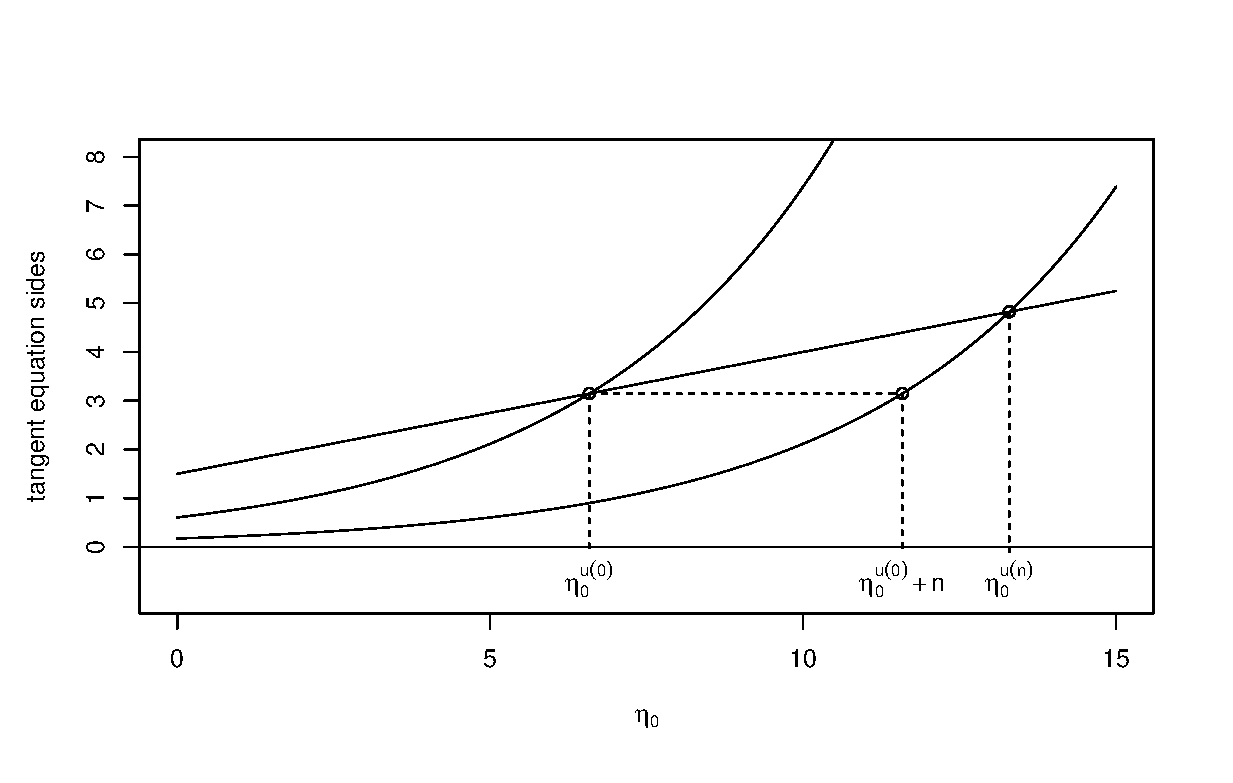
\includegraphics[trim = 48mm 35mm 49mm 47mm, clip, width=0.8\textwidth]{R/prior-vs-posterior-eta0u.eps}%
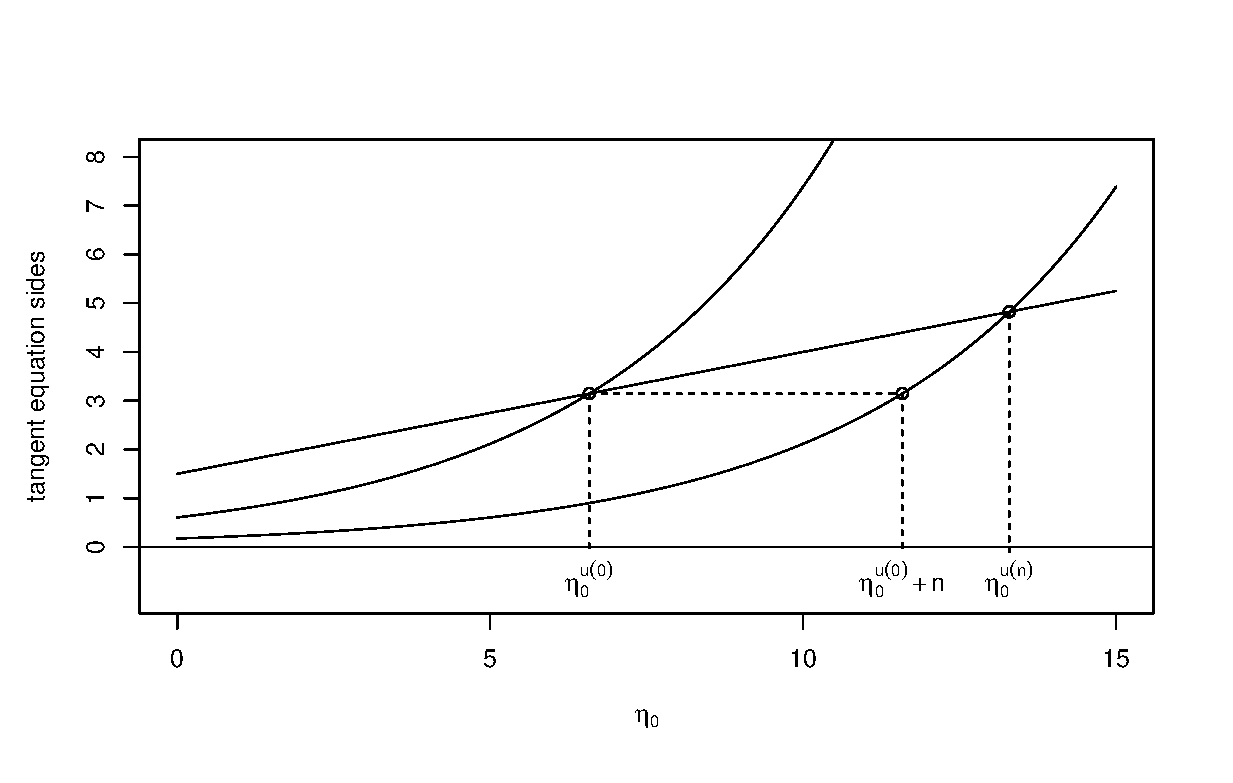
\includegraphics[trim = 1mm 5mm 10mm 20mm, clip, width=0.8\textwidth]{R/prior-vs-posterior-eta0u.eps}%
%}
\caption{Illustration for the argument that ${\eta_0^u}\un > {\eta_0^u}\uz + n$.}
\label{fig:spda1}
\end{figure}

%\subsection{Touchpoints for Update with \texorpdfstring{$s > \frac{n}{2}$}{s > n/2}}
\subsection{Touchpoints for Arbitrary Updates}
\label{sec:generalupdate}

Let us now consider the update of the basic boatshape \eqref{eq:basicset} %symmetric around the $\eta_0$ axis,
in the general case $s \neq \frac{n}{2}$,
investigating the effect that different values of $s$ for fixed $n$ have
on ${\eta_0^l}\un$ and ${\eta_0^u}\un$, %and in turn on $\ynl$ and $\ynu$.%
considering ${\eta_0^l}\un$ and ${\eta_0^u}\un$ as functions of s.%
\footnote{We will treat $s$ as a a real-valued observation in $[0,n]$
because the continuous representation is convenient for our discussions,
keeping in mind that in reality it can only take integer values.}
For $s \neq \frac{n}{2}$, $\EN$ is not symmetric to the $\ez$ axis,
and we have to derive the touchpoints ${\eta_0^l}\un$ and ${\eta_0^u}\un$ separately.
%
The upper and lower contours for $\EN$ are
\begin{align*}
\ol{c}\un(\eta_0)                   &= s - \frac{n}{2} + a - a e^{-b(\eta_0 - n - \ezl)} \,, &
%\frac{d}{d\eta_0} \ol{c}(\eta_0) &=                      ab e^{-b(\eta_0 - n - \ezl)} \,,\\
\ul{c}\un(\eta_0)                   &= s - \frac{n}{2} - a + a e^{-b(\eta_0 - n - \ezl)} \,,
%\frac{d}{d\eta_0} \ul{c}(\eta_0) &=                     -ab e^{-b(\eta_0 - n - \ezl)} \,.
\end{align*}
leading to
\begin{align}
%s - \frac{n}{2} + a - a \big(1 + b(\eta_0^u + 2)\big) e^{-b(\eta_0^u - n - \ezl)} &\stackrel{!}{=} 0 \nonumber\\
\label{eq:eta0u-general}
\frac{a}{s - \frac{n}{2} + a} \big(1 + b({\eta_0^u}\un + 2)\big) &\stackrel{!}{=} e^{b({\eta_0^u}\un - n - \ezl)} \,,\\
\label{eq:eta0l-general}
\frac{a}{\frac{n}{2} -s  + a} \big(1 + b({\eta_0^l}\un + 2)\big) &\stackrel{!}{=} e^{b({\eta_0^l}\un - n - \ezl)} \,.
\end{align}
We see thus that the graph from Fig.~\ref{fig:spda1} holds here as well,
except that the linear function on the left hand side of 
\eqref{eq:eta0u-general} and \eqref{eq:eta0l-general} is changed in slope and intercept by a factor.
(Equivalently, we can consider it to be rotated around the root $-2-\frac{1}{b}$.)
For $s=\frac{n}{2}$, this factor is 1 for both \eqref{eq:eta0u-general} and \eqref{eq:eta0l-general},
reducing to \eqref{eq:eta0uposterior}.
Due to symmetry of the prior set, we will, without loss of generality,
consider only the case $s > \frac{n}{2}$.

%\paragraph{Description of ${\eta_0^u}\un$.}

The factor $\frac{a}{s - \frac{n}{2} + a}$
in \eqref{eq:eta0u-general} is thus smaller than $1$ and decreasing in $s$.
The larger $s$, the smaller the factor, the most extreme case being $s=n$,
where the factor is $\frac{a}{\frac{n}{2} + a}$.
As the linear function's slope will be less steep (the intercept is lowered as well),
%\footnote{The common root of the linear functions for any $s$ is at $\eta_0 = -2 -\frac{1}{b}$.}
the intersection with the exponential function moves to the left,
i.e.\ ${\eta_0^u}\un(s) < {\eta_0^u}\un(\frac{n}{2})$ for $\frac{n}{2} < s < n$.
This means that $\ynu(s) > \ynu(\frac{n}{2})$.
However, ${\eta_0^u}\un(s)$ can decrease only to $\ezl+n$:
When ${\eta_0^u}\un(s)$ reaches the left end of $\EN$ at $\ezl+n$,
the gradual increase of $\ynu$ through the changing tangent slope 
%for $\ezl+n \le \eta_0^u(s) \le \eta_0^u(\frac{n}{2})$ 
is replaced by a different change mechanism,
where increase of $\ynu$ is solely due to the shift of $\EN$ in the $\eta_1$ coordinate.
Due to \eqref{eq:trafotony}, $\ynu$ is then linear in $s$.

%\paragraph{Description of ${\eta_0^l}\un$.}

In \eqref{eq:eta0l-general}, the factor to the linear function is $\frac{a}{\frac{n}{2} - s + a}$.
Here, we have to distinguish the two cases $\frac{n}{2} \le s < \frac{n}{2} + a$
and $s \ge \frac{n}{2} + a$.
In the first case, the factor is larger than $1$ and increasing in $s$.
Therefore, the intersection of the linear function with the exponential function
will move to the right, such that ${\eta_0^l}\un(s)$ becomes larger, and $\ynl$ increases.
In the second case, the factor is undefined (for $s = \frac{n}{2} + a$)
or negative (for $s > \frac{n}{2} + a$).
Either way, there is no intersection of the linear function with the exponential function
for any $\eta_0 > \ezl + n$, and %for $s \downarrow \frac{n}{2} + a$, the slope $\to \infty$.
in fact, for $s \ge \frac{n}{2} + a$, the whole set is above the $\eta_0$ axis,
and the touchpoint must be thus at $\ezu + n$.
Actually, ${\eta_0^l}\un(s) = \ezu + n$ already for some $\frac{n}{2} \le s < \frac{n}{2} + a$,
when the intersection point reaches $\ezu + n$.
At this point, gradual increase of $\ynl$ resulting from the movement of ${\eta_0^l}\un(s)$ along the set
towards the right is replaced by a linear increase in $s$.
Again, this linear increase is due to the $\eta_1$ coordinate being incremented
according to \eqref{eq:eta-update},
and from \eqref{eq:trafotony} we see that $\ynl$ is linear in $\eta_1$.


\subsection{Posterior Imprecision}
\label{sec:posteriorimprecision}

We now summarize the results from Sect.~\ref{sec:generalupdate}
and give two numerical examples.

For $s > \frac{n}{2}$, both $\ynu$ and $\ynl$ will at first increase gradually with $s$,
as ${\eta_0^u}\un$ moves to the left, and ${\eta_0^l}\un$ moves to the right.
We will call such updating of the prior parameter set
where both lower and upper posterior touchpoint are in the middle of the set as \emph{happy learning}.
\begin{figure}
\includegraphics[width=\textwidth]{R/pppboat-ipmu1.eps}
\caption{Boatshape set with $y_c = 0.5$ together with rectangle set, $1 \times [\yzl, \yzu]$ and $2 \times [\yzl, \yzu]$
with same prior imprecision (left),
and the corresponding lower and upper bounds for $\yn$ as functions of $s$ (right).}
\label{fig:ppp1}
\end{figure}
%
At some $s^u$, ${\eta_0^u}\un$ will reach $\ezl + n$,
and at some $s^l$, ${\eta_0^l}\un$ will reach $\ezu + n$.
Whether $s^l < s^u$ or vice versa depends on
the choice of parameters $\ezl, \ezu, a$ and $b$.
When $s$ is larger than either of $s^l$ or $s^u$,
we have \emph{unhappy learning},
where data $s$ is very much out of line with our prior expectations as expressed by $\EZ$.
Ultimately, when $s > s^u$ and $s > s^l$,
both $\ynu$ and $\ynl$ will increase linearly in $s$, but with different slopes.
$\ynu$ will increase with slope $\frac{1}{\ezl + n + 2}$,
whereas $\ynl$ will increase with the lower slope $\frac{1}{\ezu + n + 2}$.

These findings are illustrated in Fig.~\ref{fig:ppp1}
for a boatshape set with $y_c = 0.5$, $\ezl = -1$, $\ezu = 20$, $a=1$ and $b=0.4$. 
These are compared to a rectangular set and two line segment sets with the same $\yz$ range.
Here we see a linear increase of $\ynu$ for $s < 4$ and a superlinear increase for $s \ge 4$.
%and analogously for $\ynl$
We have thus happy learning for $s \in [4,6]$, and unhappy learning for $s \neq [4,6]$.
For $s \approx 5$, $\Delta_y$ for the boatshape set is about half of $\Delta_y$ for the rectangle set.
The line segment sets lead to very short $\yn$ ranges, but do not reflect \pdc.

Figure~\ref{fig:ppp2} depicts a numerical example for the case $y_c = 0.75$.
Notice that the rotated boatshape parameter set is not symmetric in the $(\nz, \yz)$ space.
We see that $[\ynl, \ynu]$ for the boatshape set is nearly as short as for the line segments sets
when $s \approx 0.75$, but that unlike those, the boatshape offers \pdc\ sensitivity.
Interestingly, all four sets lead to a similar $\ynl$ for $s < 5$.
\begin{figure}
\includegraphics[width=\textwidth]{R/pppboat-ipmu2.eps}
\caption{Boatshape set with $y_c = 0.75$ together with rectangle set, $1 \times [\yzl, \yzu]$ and $2 \times [\yzl, \yzu]$
with same prior imprecision (left),
and the corresponding lower and upper bounds for $\yn$ as functions of $s$ (right).}
\label{fig:ppp2}
\end{figure}


\section{Discussion and Concluding Remarks}
\label{sec:concluding}

We have described a new method for generating prior parameter sets in a conjugate setting
that, in addition to prior-data conflict sensitivity, reflect strong prior-data agreement.
%The parameter set was defined in terms of a novel parametrization \cite{2015:mik-isipta}.

Our first results decribed in this paper are encouraging,
and future studies should consider elicitation of the boatshape set parameters $\ezl, \ezu, a$ and $b$ in more detail;
pre-posterior analysis seems the most promising avenue for this.

We did not discuss the case of $y_c \neq 0.5$ in detail,
but suggested to rotate the basic set \eqref{eq:basicset} around $(-2,0)$
such that the ray of constant expectation $y_c$ forms the axis of symmetry of $\EZ$,
and gave a numerical example for this approach in Fig.~\ref{fig:ppp2}.
It would be however interesting to investigate whether another way of defining a set aligned to a certain ray could be useful,
namely by shifting $\EZ$ from \eqref{eq:basicset} in the $\eo$ dimension according to \eqref{eq:raysofconstantexpectation}.
Furthermore, alternatives to the functional form of the contour functions \eqref{eq:basiccontours} could also be worth of study,
like, e.g., the second and third quadrant's part of an ellipse $a\ez^2 + b\eo^2 = c$.

In the parameter space described in Sect.~\ref{sec:miksworld},
the update from prior parameter set to posterior parameter set
amounts to a purely data-dependent translation, leaving the set shape unchanged.
This allowed us to design a set shape according to certain desired inference properties.
The boatshape is thus just a prototypical attempt in a framework that allows
for flexible modeling of prior information and tailored posterior inference proerties,
while remaining within the generalized Bayesian paradigm.
The framework opens a wide field of research on set shapes for catering to other objectives in inference behaviour.

The method was presented here for the case of Binomial observations,
but it can be easily generalized to cover all sample distributions that belong to the exponential family,
since for all of them, a parametrization of the conjugate prior in terms of $(\ez, \eo)$ can be constructed
which again has a purely data-dependent translation as update step \cite[p.~56]{2015:mik-isipta}.


% ------------ bibliography -------------

%\section*{References}
%\printbibliography[heading=none]
\bibliographystyle{splncs03}
\bibliography{boatpaper}



\end{document}
